\documentclass[11pt]{article}
        \usepackage[margin=1in]{geometry}
        \usepackage{fontspec}
        \setmainfont{texgyretermes-regular.otf}[
            Path=/Users/gregkara/Library/TinyTeX/texmf-dist/fonts/opentype/public/tex-gyre/,
            BoldFont=texgyretermes-bold.otf,
            ItalicFont=texgyretermes-italic.otf,
            BoldItalicFont=texgyretermes-bolditalic.otf
        ]
        \usepackage{graphicx}
        \usepackage{booktabs}
        \usepackage{longtable}
        \usepackage{array}
        \usepackage{amsmath,amssymb}
        \usepackage{caption}
        \usepackage{subcaption}
        \usepackage{hyperref}
        \usepackage{placeins}
        \usepackage{pdflscape}
        \usepackage{fancyvrb}
        \usepackage{microtype}
        \hypersetup{colorlinks=true,linkcolor=blue,citecolor=blue,urlcolor=blue}

        \title{The Lexical Seam: Information-Geometric Characterization of Zipf-Mandelbrot Misspecification and a Mechanism-Capturing Discrete Alternative Family}
        \author{Grigori Karapetyan\\\small{Independent researcher; Nexus Computers LLC; Burbank, CA, USA}\\\small{Correspondence: [email]}}
        \date{}

        \begin{document}
        \maketitle

        \begin{abstract}
The Zipf-Mandelbrot (ZM) law fits word-frequency distributions accurately in the tail but consistently underpredicts at the apex. We characterize this residual mechanistically by applying deterministic enumerative symbolic regression to single-ZM residuals across 25 English corpora and 7 non-English corpora spanning four language families. The step-2 search recovers Bregman-type correction terms whose identity is organized by the single-ZM apex parameter c: the Itakura-Saito generator $(x-1)-\log(x)$ on high-c corpora and the exponential generator $\exp(x-1)-x$ on low-c corpora. The full enriched symbolic search beats the single-ZM baseline on all 25 English corpora at its terminal step, with verified RMSE improvements from 3.70\% to 25.29\% (mean 11.02\%). Synthetic mixtures of two power laws, a city-population control, and a function-word ablation localize the cause to a seam between two power-law regimes meeting at a smooth transition. The canonical rank-curve model used here is a decoupled 9-parameter two-regime ZM with an erf gate, σ(z) = [1 − erf((log r − log k)/w\_gate)]/2, and an independent tail-coordinate smoothing width w\_tail. Direct gate-family comparison under this decoupled parameterization selects the erf gate on 24/25 English corpora, with arctan winning only Dubliners; the median BIC spread across independent gates is 677 and the mean spread is 865. A falsification check on logistic-generated synthetic data recovers logistic on 25/25 corpora and never prefers erf over the true generator, indicating that the empirical erf preference is distributional structure rather than a generic fitting artifact. The smooth two-regime family absorbs the symbolic seam, while the parsimonious single-regime MOEZipf extension remains phenomenologically competitive but leaves Bregman-shaped residual structure. Simulation recovery from fitted smooth models provides causal support for the two-regime mechanism; on the low-c side, recovery is geometric rather than formula-unique because $\exp(x-1)-x$ and $x^x-\sqrt{x}$ lie on a near-degenerate head manifold. The previously tight transition-centre scaling claim weakens under the decoupled erf model: log(k\_erf) regressed on log(V) gives β = 0.758 with 95\% CI [0.346, 1.171] and $R^2$ = 0.386. This interval includes the coupled-logistic estimate 0.521 and the POS crossover estimate 0.545, but the canonical model shows substantial cross-corpus variability not captured by a simple log-linear law. We further formulate a discrete finite-support Seam-Mandelbrot PMF fit by maximum likelihood on token counts; under 80/20 binomial splits the soft-k-regularized variant beats MOEZipf on 17/25 corpora on full held-out average negative log-likelihood (median advantage −0.00195) and absorbs the symbolic seam on 21/25 residuals. The two-regime structure generalizes across all 32 corpora; Bregman-type generators win step-2 on all 29 Indo-European alphabetic corpora under the original grammar, while very-low-c Russian, Mandarin, and Arabic select $x^x-\sqrt{x}$ in a manner consistent with the same low-c manifold. We position the Bregman residual as a diagnostic biomarker for single-regime misspecification, the decoupled erf two-regime model as the current canonical rank-curve mechanism, and the Seam-Mandelbrot PMF as a mechanism-capturing discrete alternative to parsimonious phenomenological skew extensions.

\end{abstract}
\section{Introduction}\label{sec:intro}

The rank-frequency distribution of words in a natural language corpus is a canonical empirical regularity. Zipf~\cite{zipf1949} observed that the frequency f\_r of the r-th most common word is approximately proportional to 1/r. Mandelbrot~\cite{mandelbrot1953} generalized this to a three-parameter form,

\begin{equation}
\tag{1}\label{eq:zm}
f_r \approx a \cdot (r + c)^{-b},
\end{equation}

which adds a linear shift c that flattens the apex and more closely matches empirical rankings. The resulting Zipf-Mandelbrot law has served as a baseline model for several decades in quantitative linguistics, information theory, and the statistics of complex systems.

Despite its broad applicability, ZM exhibits systematic residuals at the apex of empirical rank-frequency distributions. The most frequent words are consistently underfit by equation (1) when b, c, and a are estimated by nonlinear least squares on log-transformed rank and frequency. Two prior lines of work address this deficit. Ferrer-i-Cancho and Solé~\cite{ferrer2001} proposed that natural language corpora comprise two distinct power-law regimes, interpreted as a core lexicon of high-frequency function words and a larger content-word lexicon. Pérez-Casany and Casellas~\cite{perez2013} proposed the Marshall-Olkin Extended Zipf (MOEZipf) distribution, which adds a single skewing parameter β to the Zipf family and produces concave or convex deformation of the apex while preserving linear tail behaviour. Both improve empirical fit; neither characterizes the functional form of the residual from a first-principles derivation.

Symbolic regression (SR) provides a different methodology. Rather than positing a parametric correction and fitting its coefficients, SR searches over candidate algebraic expressions and selects those that minimize a data-fit objective. Modern SR implementations use genetic programming (Cranmer~\cite{cranmer2023}; Schmidt and Lipson~\cite{schmidt2009}), reinforcement learning with recurrent policies (Petersen et al.~\cite{petersen2020}), brute-force polynomial enumeration with symmetry detection (Udrescu and Tegmark~\cite{udrescu2020}), and transformer-based equation decoders (Biggio et al.~\cite{biggio2021}; Kamienny et al.~\cite{kamienny2022}). Applied to classical physics, these methods have rediscovered known laws from data. Their application to ZM residuals on real linguistic corpora has not, to our knowledge, been reported.

We apply a deliberately minimal SR variant — a deterministic enumerative beam search seeded only with the variable x and the integer 1 — to the ZM residual across 25 English corpora. Restricting to parameter-free symbolic expressions eliminates floating-point curve fitting and ensures that any discovered structure reflects algebraic composition rather than tuning of continuous coefficients. We examine the dominant discovered expressions through the lens of information geometry, verify the resulting mechanistic hypothesis with non-linguistic controls, synthetic mixtures, and an independent part-of-speech analysis, compare two-regime parameterizations against MOEZipf under Bayesian Information Criterion, distinguish these models mechanistically by testing which absorb the symbolic seam, derive the local form of the smooth-model seam analytically, perform a simulation recovery experiment to test causal sufficiency, characterize the low-c regime as a near-degenerate head manifold, and extend the pipeline to seven non-English corpora.

The evidence is organized around four pillars. First, the single-ZM residual is Bregman-divergence-shaped across English corpora, and the full enriched symbolic search improves over single ZM on 25/25 corpora at its terminal step. Synthetic controls and function-word ablations establish this shape as a diagnostic consequence of fitting a single curve to a two-regime population. Second, a smooth two-regime ZM family absorbs the symbolic seam and dominates hard or continuous break models on the same corpora; MOEZipf remains a strong phenomenological competitor but does not absorb the mechanism. Third, the smooth transition is not merely generic smoothness: under a decoupled 9-parameter parameterization, direct gate-family comparison selects an erf gate on 24/25 English corpora, and a logistic-generated synthetic recovery check recovers logistic on 25/25 rather than spuriously preferring erf. Fourth, simulation recovery from fitted smooth models provides causal support for the mechanism, with exact high-c recovery and geometric low-c recovery on a near-degenerate head manifold. The discrete Seam-Mandelbrot PMF then transfers the same mechanism into likelihood space under an explicit scope condition: corpora should be single coherent two-regime samples, not aggregate anthologies.

We frame the Bregman residual as a diagnostic biomarker for single-regime misspecification and the decoupled erf two-regime model as the current canonical rank-curve explanation of the underlying structure.

\section{Methods}\label{sec:methods}

\subsection{Corpora}

We assembled 25 English-language corpora from Project Gutenberg spanning six centuries of literary composition. Corpora cover a range of genres, authorship structures, and vocabulary sizes (V = 3,814 for Principia Ethica through V = 28,990 for Ulysses). Preprocessing consisted of lowercasing, tokenization on Unicode word boundaries, and removal of metadata headers and footers supplied by Project Gutenberg. Seven non-English corpora (Russian, Mandarin, Arabic, Latin, French, Spanish, Dutch; details in Section 3.10) used the same pipeline with language-appropriate tokenization where necessary (jieba for Mandarin; Unicode-aware regex for the others).

\subsection{Single-curve Zipf-Mandelbrot baseline}

For each corpus we computed the rank-frequency distribution and fit equation (1) by nonlinear least squares on log-transformed frequencies, minimizing

\begin{equation}
\tag{2}\label{eq:ols}
\sum_r \left[\log(f_r) - \log(a) + b \cdot \log(r + c)\right]^2
\end{equation}

over (a, b, c). The residual e\_r is

\begin{equation}
\tag{3}\label{eq:residual}
e_r = \log(f_r) - \log(a) + b \cdot \log(r + c).
\end{equation}

\subsection{Normalization of the rank axis}

To produce a bounded input variable for symbolic regression, we normalized log-rank via

\begin{equation}
\tag{4}\label{eq:xnorm}
x = 0.05 + 0.95 \cdot \log(r) / \log(V),
\end{equation}

mapping log-rank onto [0.05, 1.0] while preserving log-log linear structure. We verified that the dominant discovered expressions, when re-expressed in original log-rank coordinates, depend only on the corpus-specific constant log(V) and preserve their functional form across corpora with different vocabulary sizes.

\subsection{Deterministic enumerative symbolic regression}\label{sec:srmethod}

We applied a deterministic enumerative beam search to the residual signal e\_r(x). The search operates on the grammar

\begin{equation}
\tag{5}\label{eq:grammar}
S \to 1 \mid x \mid u(S) \mid b(S,S)
\end{equation}

where u $\in$ \{neg, inv, sqr, sqrt, exp, log\} are unary operators and b $\in$ \{add, sub, mul, div, pow\} are binary operators. A user-defined binary operator eml(a, b) = exp(a) − log(b), recently shown by Odrzywolek~\cite{odrzywolek2026} to generate all elementary functions under composition with the constant 1, was included for completeness; it does not appear in any of the dominant discovered expressions we report.

At each step, candidates are generated by applying every applicable operator to every pair (or singleton) of expressions in the current vocabulary. Candidates that produce NaN, infinity, or constant output are rejected. Surviving candidates are deduplicated by value signature: two expressions with numerically equal output vectors (rounded to ten decimal places) are considered equivalent and the shorter abstract syntax tree is retained. After deduplication, a diverse beam of the top 50 candidates is selected by a weighted blend of in-sample RMSE and structural dissimilarity of abstract syntax trees. The beam is carried to the next step. We execute 10 steps and retain the full step-2 beam without truncation for subsequent analysis.

This is a standard configuration of enumerative SR with semantic hashing and structural diversity pruning. It contains no learned parameters, no genetic-programming mutation or crossover, and no continuous coefficient optimization inside selected expressions. By restricting the search to parameter-free algebraic composition seeded only with x and 1, any selection of a given expression reflects intrinsic fit to the residual rather than tuning of floating-point constants.

\subsection{Auxiliary single-regime baseline: MOEZipf}

For comparison against a published single-regime extension, we fit the Marshall-Olkin Extended Zipf distribution of Pérez-Casany and Casellas~\cite{perez2013}:

\begin{equation}
\tag{6}\label{eq:moe}
P(Y = k) = k^{-\alpha} \cdot \beta \cdot \zeta(\alpha) / [(\zeta(\alpha) - \bar{\beta}\cdot \zeta(\alpha,k)) \cdot (\zeta(\alpha) - \bar{\beta}\cdot \zeta(\alpha,k+1))]
\end{equation}

where ζ(α) is the Riemann zeta function, ζ(α, k) is the Hurwitz zeta function, and β̄ = 1 − β. Parameters α and β were fit by maximum likelihood; the corresponding rank-curve RMSE on log-frequencies places MOEZipf on a common footing with the piecewise and smooth-transition models.

\subsection{Two-regime parameterizations}

We evaluated two families of two-regime ZM parameterizations. The first family tests whether a two-regime transition is needed at all; the second tests which smooth gate is empirically preferred once the transition coordinate is decoupled from the tail-coordinate smoothing scale.

\paragraph{Hard piecewise:} two independent ZM fits on rank windows [1, K] and [K+1, V] with K = 500.

\paragraph{Continuous piecewise:} two ZM curves constrained to intersect at a shared breakpoint K, so that

\begin{equation}
\tag{7}\label{eq:continuity}
a_1 - b_1 \cdot \log(K + c_1) = a_2 - b_2 \cdot \log(K + c_2).
\end{equation}

The breakpoint K was optimized by grid search over integer rank values because the piecewise mask is a step function with zero continuous gradient. For each candidate K, the remaining five continuous parameters ($a_1$, $b_1$, $c_1$, $b_2$, $c_2$) were fit by nonlinear least squares.

\paragraph{Canonical decoupled smooth model (9-parameter):} a smooth blend of two ZM curves,

\begin{equation}
\tag{8}\label{eq:sigmoid}
\log f_r = \sigma_r \cdot \mathrm{ZM}_1(r) + (1 - \sigma_r) \cdot \mathrm{ZM}_2(\rho_{\mathrm{tail}}(r; k, w_{\mathrm{tail}}))
\end{equation}

\begin{equation}
\tag{9}\label{eq:sigmoid-gate}
\sigma_r = [1-\operatorname{erf}((\log r-\log k)/w_{\mathrm{gate}})]/2
\end{equation}

with free parameters ($a_1$, $b_1$, $c_1$, $a_2$, $b_2$, $c_2$, k, w\_gate, w\_tail). The head branch is $\mathrm{ZM}_1$(r) = $a_1$ − $b_1$ log(r + $c_1$). The tail branch is $\mathrm{ZM}_2$(ρ\_tail + $c_2$) = $a_2$ − $b_2$ log(ρ\_tail(r; k, w\_tail) + $c_2$), where

ρ\_tail(r; k, w\_tail) = 1 + s · log(1 + exp((r − k) / s)),   s = max(1, k · w\_tail).

The decoupling is deliberate: w\_gate controls the steepness and tail behavior of the transition gate, while w\_tail controls the smooth local rank coordinate on which the tail ZM is evaluated. Coupled fits used a single width for both roles; Section 3.5 reports that the decoupled erf model is the canonical smooth rank-curve model used below.

\paragraph{Gate-family comparison:} to test whether the transition is specifically erf-shaped or merely smooth, we fit the same 9-parameter model with five gates: logistic, tanh, erf, algebraic, and arctan. The independent gates are logistic, erf, algebraic, and arctan; tanh is included as an optimizer calibration because it is exactly equivalent to logistic under the reparameterization w\_tanh = 2w\_logistic. The gate functions were:

σ\_logistic(z) = 1 / (1 + exp(z / w\_gate))

σ\_tanh(z) = [1 − tanh(z / w\_gate)] / 2

σ\_erf(z) = [1 − erf(z / w\_gate)] / 2

σ\_algebraic(z) = [1 − z / sqrt(w\_gate² + z²)] / 2

σ\_arctan(z) = 0.5 − arctan(z / w\_gate) / π,

where z = log r − log k for algebraic and arctan, and z is divided by w\_gate inside the logistic, tanh, and erf expressions as written above. Fits used 100 random starts of a trust-region nonlinear least-squares optimizer. Decoupled bounds were $a_1$, $a_2$ $\in$ [−100, 100]; $b_1$, $b_2$ $\in$ [0.5, 3.0]; $c_1$, $c_2$ $\in$ [0, 1000]; k $\in$ [20, 2000]; w\_gate $\in$ [0.05, 10.0]; w\_tail $\in$ [0.05, 10.0]. We saved per-start dispersion, bound-hit flags, and tanh/logistic calibration diagnostics for the gate-family sweep.

\subsection{Bayesian Information Criterion}

For each model and corpus,

\begin{equation}
\tag{10}\label{eq:bic}
\mathrm{BIC} = p \cdot \log(n) + n \cdot \log(\mathrm{MSE})
\end{equation}

where p is the number of free parameters, n is the vocabulary size, and MSE is the mean squared residual of log-frequencies versus model predictions. Lower BIC indicates preferred fit under the combined criteria of likelihood and parsimony. BIC comparisons appear in Section 3.5.

\subsection{Synthetic mixture protocol}

To test whether Bregman-shaped residuals are specific to natural language or arise from any two-regime power-law mixture, we generated synthetic rank-frequency data from mixtures of two discrete Pareto distributions with tail exponents $\alpha_1$ and $\alpha_2$ and relative weight $w_1$. For each configuration we computed the rank distribution of the sum of the two populations, fit single-ZM, and ran the enumerative search on the resulting residual. Four configurations were tested: ($\alpha_1$, $\alpha_2$) = (1.5, 1.3), (1.5, 0.8), (1.5, 0.5), and (1.5, 1.5) as a same-exponent control.

\subsection{Part-of-speech crossover analysis}

For each English corpus, we POS-tagged the full text using spaCy en\_core\_web\_sm and assigned each distinct word type to a corpus-majority POS tag. Closed-class tags were ADP, AUX, CCONJ, DET, PART, PRON, SCONJ. Open-class tags were ADJ, ADV, NOUN, PROPN, VERB. For the top 500 word types ordered by corpus frequency, we computed the running fraction of closed-class types from rank 1 through rank r and identified the rank $k_{\mathrm{POS}}$ at which this running fraction first crosses 0.50. We additionally performed manual POS classification on the top 300 types of Shakespeare, Moby Dick, Federalist Papers, and Wealth of Nations to cross-check spaCy outputs; manual and automated crossovers agreed to within 15 ranks on all four corpora.

\subsection{Residual symbolic search after baseline models}

To test whether competing baseline models absorb the structure that step-2 detects on single-ZM residuals, we applied the enumerative search of Section 2.4 to residuals of two alternative baselines: MOEZipf (Section 2.5) and the smooth two-regime model (Section 2.6). For each corpus and each baseline, the residual was log f\_r minus the baseline prediction; the search ran with identical configuration. Helpful corrections were defined as step-2 formulas producing composite RMSE improvement greater than 0.001 in log-frequency over the baseline alone.

\subsection{Head-focused RMSE and local residual basis fit}

To distinguish head-of-distribution structure from tail fluctuations, we defined head-only RMSE metrics restricted to the top 50, 100, and 200 ranks. Candidate step-2 expressions were rescored under each head metric and winner identities compared to full-corpus winners. We fit the three-term local basis

\begin{equation}
\tag{11}\label{eq:head-basis}
e_r = a_1 \cdot (1 - x) + a_2 \cdot (1 - x)^2 + a_3 \cdot (1 - x)^3
\end{equation}

to the empirical ZM residual over the top 200 ranks of each corpus by ordinary least squares. The basis spans the local head residual geometry in the normalized log-rank coordinate of Section 2.3.

\subsection{Analytic seam derivation}

We wrote the smooth two-regime prediction in head log-rank coordinates z = log(r) − log(k) as

\begin{equation}
\tag{12}\label{eq:seam-form}
Y(z) = Y_{\mathrm{head}}(z) + \tau(z)\cdot \Delta(z)
\end{equation}

where Y\_head is the head-regime ZM curve, Δ(z) = $\mathrm{ZM}_2$(z) − $\mathrm{ZM}_1$(z) is the regime gap, and τ(z) = 1 − σ(z) is the tail-regime activation from equation (9). For the canonical erf gate, τ(0) = 1/2, τ'(0) = 1/(√π w\_gate), τ''(0) = 0, and τ'''(0) = −2/(√π w\_gate³). We Taylor-expanded the seam term τ(z) · Δ(z) at z = 0 and computed the first three centered coefficients analytically (equations 16–18, Section 3.8). We further derived the first-order tangent-space projection of the seam onto the head-branch ZM parameter manifold (equation 19, Section 3.8) using tangent basis vectors g\_a(r) = 1, g\_b(r) = −log(r + $c_1$), g\_c(r) = −$b_1$/(r + $c_1$). The algebraic form of this projection is gate-independent; coupled-logistic numerical sign checks are not transferred to the decoupled erf parameterization without rerunning the sign-validation experiment.

\subsection{Simulation recovery protocol}

To test causal sufficiency of the smooth two-regime model as a generative explanation for the empirical symbolic signal, we performed a simulation recovery experiment. For each English corpus, we used the fitted smooth model (Section 2.6) to generate synthetic rank-frequency data: we evaluated the smooth-model predicted log-frequencies at the empirical rank values, exponentiated, sampled integer counts from a Poisson distribution at each rank to match the stochasticity of real corpora, and recomputed the rank-ordered distribution. We repeated the procedure as a control using synthetic data from the fitted single-ZM baseline (Section 2.2). For both, we ran the complete analysis pipeline used on empirical data: single-ZM refit, step-2 enumerative search, head-basis fit, and head-only metric scoring. Summary outputs (winner identity, step-2 help rate, head-basis coefficients, Euclidean head-only gap) were compared to empirical outputs to quantify recovery. We additionally ran a gate-recovery falsification test in which logistic-generated synthetic corpora were refit by the five-gate decoupled model family; this test checks whether the empirical erf preference can be produced as a generic fitting artifact.

\subsection{Low-c head manifold analysis and synthetic parameter sweep}

For English corpora with empirical full-RMSE step-2 winner $\exp(x-1)-x$ (14 corpora), we characterized the local geometry of candidate step-2 generators on the head of the distribution. For each corpus and head window (top 100, top 200), we computed: (i) the cosine similarity between evaluated vectors of $\exp(x-1)-x$ and $x^x-\sqrt{x}$; (ii) the coefficient of determination $R^2$ of OLS fits of the empirical head residual onto two-dimensional spans \{exp, $x^x-\sqrt{x}$\} and \{exp, IS\}; (iii) the ordering of four candidate generators \{IS Bregman, exp Bregman, Euclidean, $x^x-\sqrt{x}$\} under each metric; (iv) pairwise RMSE differences between $\exp(x-1)-x$ and $x^x-\sqrt{x}$ on full-curve and head-only metrics.

To identify which smooth-model parameters control the orientation of the low-c head manifold, we ran a synthetic parameter sweep in the coupled smooth family that preceded the decoupled erf gate-family comparison. We constructed smooth models on a grid varying transition fraction (the normalized rank position of k), transition width, and tail-versus-head slope contrast ($b_2$ − $b_1$), holding other parameters fixed at empirical low-c medians. For each grid point we generated synthetic data via the protocol of Section 2.13, ran the full pipeline, and computed: (a) the manifold orientation θ defined as the angle of the empirical head residual when projected onto the \{exp, $x^x-\sqrt{x}$\} basis; (b) the head-weight λ\_flip at which the step-2 winner switches from exp to $x^x-\sqrt{x}$ as the head weight is varied from 0 (full RMSE) to 1 (top-100 only). Pearson correlations of θ and λ\_flip with each smooth-model parameter quantified the primary controls. The decoupled erf model separates w\_gate from w\_tail; parameter-correlation claims involving "width" are therefore interpreted as coupled-family diagnostics unless explicitly rerun under the decoupled model.

\subsection{Multi-language pipeline}

The multi-language extension (Section 3.10) used the same pipeline as the English analysis with language-specific tokenization: jieba word segmentation for Mandarin; whitespace-plus-Unicode tokenization for Russian, Arabic, French, Spanish, Dutch, and Latin. Corpus sources were Wikisource (Russian War and Peace, Arabic One Thousand and One Nights) and Project Gutenberg (Mandarin Romance of the Three Kingdoms, Latin De Bello Gallico, French Les Misérables, Spanish Don Quijote, Dutch Max Havelaar). For corpora exceeding approximately 150,000 tokens in raw form, we used a leading 150,000-token slice for computational feasibility; this truncation does not change rank orderings in the vocabulary slice used for ZM fitting. Parameter bounds and search configurations were identical to the English analysis.

\subsection{Seam-Mandelbrot probability mass function}\label{sec:pmf}

The smooth-transition two-regime model of Section 2.6 was formulated first as a rank-curve fit in log-frequency space. To compare mechanism capture directly with MOEZipf's likelihood-space objective, we formulated the discrete Seam-Mandelbrot probability mass function (PMF) by normalizing a smooth seam over the finite rank support [1, V]:

\begin{equation}
\tag{20}\label{eq:pmf-unnorm}
P_{\mathrm{SM}}(r \mid \theta) = \exp[S(r;\theta)] / Z(\theta),
\end{equation}

\begin{equation}
\tag{21}\label{eq:pmf-Z}
Z(\theta) = \sum_{r=1}^{V} \exp[S(r;\theta)],
\end{equation}

where S(r; θ) is the smooth-seam log-frequency prediction evaluated at rank r. The likelihood-space PMF experiments reported in Section 3.11 use the six-parameter Seam-Mandelbrot variant already fit on binomial train/test splits, with amplitudes absorbed into the normalization constant. They establish that a smooth two-regime seam can be transferred into probability-mass space; the gate-family specificity result in Section 3.5 is a separate rank-curve analysis under the decoupled erf parameterization.

PMF parameters were fit by maximum likelihood on train-partition token counts, with an 80/20 train/test split generated by binomial splitting of each type count independently. Held-out performance was evaluated as average negative log-likelihood per held-out token under the fitted PMF. For comparison against published baselines, we fit truncated Zipf, truncated Zipf-Mandelbrot, and truncated MOEZipf PMFs under identical train/test protocol.

\subsection{Regularization study on PMF parameters}

The free 6-parameter PMF fit exhibits overfitting on binomial splits of moderate-sized corpora. To test whether parameter pooling improves generalization, we evaluated three regularization variants of the Seam-Mandelbrot PMF: (i) fixed-k, in which k is constrained to $V^{\alpha}$ with α = 0.521, the coupled-model pooled exponent used when these PMF experiments were run; (ii) fixed-k,w, in which both k = $V^{\alpha}$ and w = 0.990, a pooled central value from the fitted smooth family, are fixed; (iii) soft-k, in which the train objective adds a quadratic penalty λ\_k · (log k − α log V)² with α = 0.521 and λ\_k selected per corpus from the grid \{1e-4, 3e-4, 1e-3, 3e-3, 1e-2, 3e-2\}. We additionally evaluated an empirical-Bayes hierarchical variant in which log k\_i ~ Normal(α log V\_i, σ²) with α and σ fit jointly across all corpora by iterative expectation-maximization, and an asymmetric-gate variant in which the single width w is replaced by (w\_left, w\_right) permitting distinct seam widths on either side of the transition.

\subsection{Per-book anthology decomposition}

To test the structural basis of aggregate-level fitting failures on anthology corpora, we decomposed the King James Bible into its canonical 66 books (Protestant canon) and fit the soft-k Seam-Mandelbrot PMF independently to each book. We computed per-book step-2 gains on fitted-model residuals, per-book held-out average NLL against ZM and MOEZipf baselines under identical 80/20 binomial splits, and aggregate per-book held-out NLL weighted by test-token counts. The aggregate was compared directly to the whole-Bible single-fit held-out NLL to quantify the generalization improvement from respecting the single-two-regime assumption at the appropriate unit of analysis.

\subsection{Hybrid head-tail and fully-ours nested seam architectures}

Two extensions to the Seam-Mandelbrot PMF were evaluated as likelihood-focused alternatives (Section 3.11). The hybrid head-tail PMF defines a discrete PMF P\_H(r | θ) = [σ(r; k, w) · P\_ZM(r | $b_1$, $c_1$) + (1 − σ(r; k, w)) · P\_MOE(r | $b_2$, $c_2$, α)] / Z(θ), where σ is the smooth seam gate used in the PMF family, P\_ZM is the standard Zipf-Mandelbrot PMF over ranks, P\_MOE is the MOEZipf PMF of Pérez-Casany and Casellas~\cite{perez2013}, and Z(θ) normalizes the sum over [1, V]. Parameters ($b_1$, $c_1$, $b_2$, $c_2$, α, k, w) are fit by MLE under the soft-k regularization of Section 2.17.

The fully-ours nested seam variant replaces the imported MOEZipf tail component with a second ZM component and embeds a fixed mini-seam within the head regime. The full parameterization is an 8-parameter model with free ($b_1$, $c_1$, $b_2$, $c_2$, $b_3$, $c_3$, k, w), where ($b_1$, $c_1$) parameterize the first head-regime ZM, ($b_2$, $c_2$) parameterize the second head-regime ZM, ($b_3$, $c_3$) parameterize the tail ZM, and (k, w) parameterize the main seam gate. The mini-seam between the two head-regime ZMs is fixed with position $k_0$ = max(5, 0.5 · log V) and width $w_0$ = 0.22. Additive amplitude parameters are absorbed into the normalization constant Z(θ) as in the base Seam-Mandelbrot PMF. A three-regime variant with three ZM components blended sequentially by two smooth gates is also evaluated as a comparison. All variants are fit by MLE under the canonical 80/20 binomial split protocol with parameter initialization seeded from soft-k and single-ZM fits augmented by random starts within bounds (b $\in$ [0.05, 5.0], c $\in$ [0, 5000], w $\in$ [0.05, 5.0]).

\subsection{Step-10 ablation and polynomial decomposition}

To test whether deeper symbolic search reveals additional interpretable structure beyond the step-2 Bregman finding, we ran our deterministic enumerative beam search to depth 10 on two exemplar high-c corpora (Shakespeare and War and Peace). Beam width and semantic-hash pruning are identical to the step-2 protocol. Step-10 dominant formulas are saved as symbolic expression trees. To quantify the structural content of the incremental step-10 correction, we evaluated (step10 − step2) on a 1000-point uniform grid of normalized x in [0.05, 0.95] and fit least-squares polynomials of degrees 3, 4, and 5. Additionally we fit a composite residual model of the form ZM + [$(x-1)-\log(x)$] + poly\_d(x) directly on full-corpus residuals with d $\in$ \{3, 4, 5\} and compared its RMSE to the step-10 monster's RMSE on each corpus. Polynomial coefficients were saved and evaluated for cross-corpus transfer (Shakespeare → War and Peace, War and Peace → Shakespeare and King James Bible, Moby Dick → Bible).

\subsection{Grammar-widening diagnostic}

To test the robustness of the step-2 Bregman finding to grammar choice, we extended the unary operator set to include \{sin, cos, tan, sinh, cosh, tanh, erf, gamma, Bessel J0\} alongside the existing operators \{neg, inv, sqr, sqrt, exp, log\}. Binary operators and atoms (x, 1) were unchanged. All other search parameters (beam width, semantic hashing, structural diversity, no continuous coefficient fitting, seeds) matched the standard protocol. The widened search was executed at step 2 (for comparison to the canonical step-2 finding) on Shakespeare, War and Peace, and Pride and Prejudice as the initial diagnostic. An extended version covered 14 English low-c corpora plus three non-English c $\approx$ 0 corpora (Russian, Mandarin, Arabic), totaling 17 low-c corpora.

For manifold-membership testing, the widened step-2 winner f\_w(x) on each corpus was tested for membership in the 2D span of \{f\_exp(x) = $\exp(x-1)-x$, f\_xx(x) = $x^x-\sqrt{x}$\}. We computed weighted centered cosine similarity between f\_w and each of \{f\_exp, f\_xx\} on the top-200 head region with empirical frequency weights, and the weighted centered 2D-span $R^2$ of f\_w in the span of \{f\_exp, f\_xx\}. A verdict of "yes" (manifold membership confirmed) was assigned at span $R^2$ > 0.9.

\section{Results}

\subsection{Bregman divergences dominate the ZM residual across English corpora}\label{sec:3-1-bregman}

Across all 25 English corpora, the deterministic search exposes the same Bregman-type step-2 diagnostic family, but the improvement claim depends on which search depth is being summarized. At step 2, the winning expression is one of two Bregman generators on 25 of 25 corpora, but the raw step-2 correction is not uniformly helpful: it improves over single ZM on 12/25 corpora, with positive gains from 0.33\% to 2.50\%, and has a median all-corpus improvement of −0.23\%. The terminal enriched search, by contrast, improves over single ZM on 25/25 corpora, with verified improvements from 3.70\% to 25.29\% and mean 11.02\%. We therefore treat step 2 as the interpretable diagnostic lens and the terminal search as the fit-improvement metric. The step-2 diagnostic expressions are:

- On corpora with larger ZM c parameter (c above approximately 79 in our sample), the dominant expression is (x − 1) − log(x), the generator of the Itakura-Saito Bregman divergence, obtained from the convex function φ(x) = −log(x) via φ(x) − φ(1) − φ'(1)(x − 1).

- On corpora with smaller ZM c parameter (c below approximately 66), the dominant expression is exp(x − 1) − x, the generator of the exponential Bregman divergence, obtained from φ(x) = exp(x) via the same construction.

The c-value bands are empirical, not a sharp threshold. In a narrow intermediate range, both expressions are near-tied and the ranking is sensitive to the normalization boundary x\_low (Section 2.3). Both expressions are present in the step-2 beam on all 25 corpora. The verified mean step-2 RMSE gap between the winner and the runner-up is 0.00201 in log-frequency; the terminal final-step mean winner-runner gap is 0.00075. Table~\ref{tab:zm-params} reports per-corpus ZM parameters, step-2 winners, and RMSE improvements.

The two Bregman generators are related by convex conjugation: the Itakura-Saito generator φ(x) = −log(x) and the exponential Bregman generator φ(x) = exp(x) satisfy φ*(y) = φ(−y) under Legendre-Fenchel duality on the appropriate domain. Geometrically, the ZM residual takes the form of a local distance measure on a curved probability manifold rather than on Euclidean space, with the specific manifold geometry switching depending on the ZM apex parameter c.

Five robustness tests verified the finding. First, the Euclidean Bregman generator (1 − x)², reachable by the same search in the same number of steps, was never the step-2 winner on any corpus. The median RMSE gap between the winning expression and (1 − x)² is 0.006 in log-frequency, placing Euclidean close to but consistently below the selected Bregman-type generators. The step-2 beam contains a tight family of candidate expressions (Euclidean, Itakura-Saito, exponential Bregman, (1 − x)·log(x), and related convex forms) whose RMSEs are typically within 0.01 of each other; the consistent ranking below Bregman forms is informative but not a large-margin separation under full-RMSE scoring. Section 3.7 shows the apparent tightness is a tail-dominance scoring artifact; head-only metrics produce clean separation. Second, an ablation of exponentiation-clamp and value-magnitude guards (EXP\_CLAMP $\in$ \{20, 30, 60\}; VALUE\_ABS\_LIMIT $\in$ \{$10^4$, $10^6$, $10^9$\}) produced identical step-2 winners. Third, an ablation of the normalization boundary x\_low $\in$ \{0.01, 0.05, 0.10\} produced stable winners on corpora away from the c-transition region; near the transition, the ranking of Itakura-Saito versus exponential Bregman flipped between neighbouring boundary settings. Fourth, a weighted-least-squares variant of equation (2) using rank-proportional weights reduced the magnitude of the improvement by approximately 50\% but did not alter winner identity on any corpus. Fifth, both Bregman-type winning expressions satisfy the three defining boundary conditions of a Bregman divergence generator at x = 1: C(1) = 0, C'(1) = 0, and C''(x) > 0 over (0, $\infty$). The Euclidean form (1 − x)² also satisfies these conditions, as expected for a valid Bregman generator on its own domain; the empirical result is that the selected generators consistently outperform the Euclidean form in this domain.

\input{tables/table1.tex}

\begin{figure}[t]
\centering
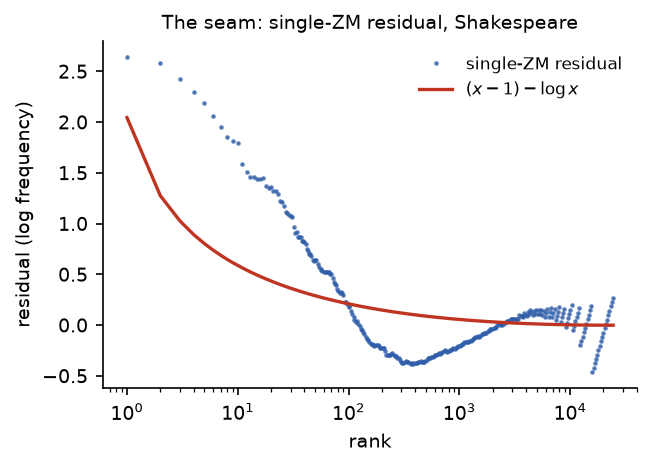
\includegraphics[width=0.9\linewidth]{figures/fig1_residual.png}
\caption{Single-ZM residual with the step-2 Bregman overlay on Shakespeare.}
\label{fig:residual}
\end{figure}

\begin{figure}[t]
\centering
\includegraphics[width=0.9\linewidth]{figures/fig2_seam_gallery.png}
\caption{Four-corpus seam gallery (high-c, mid-c, low-c, very-high-c).}
\label{fig:seamgallery}
\end{figure}

\subsection{Non-linguistic control: Bregman pattern is absent in city population data}

Applied to a worldwide city population dataset (33,535 cities, V = 33,535, single-ZM c = 100.4), the pipeline produces single-ZM RMSE 0.1206. The step-2 beam contains both Bregman generators, but the step-2 winner fails to improve over the single-ZM baseline: composite RMSE 0.1225, higher than baseline. The city-population distribution is adequately described by a single-regime ZM; the residual contains no Bregman-shaped correction that improves fit.

This eliminates the hypothesis that Bregman residuals are an artifact of enumerative search on any Zipfian data. The pattern is specific to the linguistic corpora in our sample.

\subsection{Function-word ablation localizes the effect to the seam}

Two ablations on Shakespeare. Removing the top 100 most frequent words and refitting single-ZM produced c = 607.1 with the exponential Bregman generator as the step-2 winner but the correction failing to improve RMSE. Removing the top 50 produced c = 454.1 with Itakura-Saito as the still-helping step-2 winner. Fitting single-ZM to only the top 100 words produced c = 5.3 with RMSE 0.044 and no helpful step-2 correction: the function-word-only distribution is adequately described by a single ZM.

Function words alone, as an isolated population, obey a ZM law without Bregman-shaped residual. Content words alone, as an isolated population, also follow a ZM law without helpful Bregman correction. The residual appears when the two populations are fit together by a single curve, where the transition between them produces the geometric deficit.

\subsection{Synthetic mixtures reproduce the Bregman residual}

Synthetic rank-frequency data was generated from mixtures of two discrete Pareto distributions per Section 2.8. For the same-exponent control ($\alpha_1$ = $\alpha_2$ = 1.5), the synthetic distribution is a pure power law; ZM produces a trivially good fit and no Bregman-shaped correction appears.

For the small-gap mixture ($\alpha_1$ = 1.5, $\alpha_2$ = 1.3, $w_1$ = 0.5), the step-2 winner is (x − 1) − log(x), the Itakura-Saito generator, and the correction reduces residual RMSE. The synthetic mixture reproduces the Bregman pattern observed on natural language corpora.

For medium-gap and large-gap mixtures ($\alpha_2$ = 0.8 and $\alpha_2$ = 0.5), alternative correction terms appear at step 2, consistent with two-component structure but not specifically the Itakura-Saito form.

The small-gap synthetic result establishes that Bregman-shaped ZM residuals are the geometric footprint of fitting a single analytical curve over a two-regime power-law mixture. The relationship does not depend on natural language data, lexical structure, or any linguistic mechanism; it follows from the algebraic composition of two overlapping power laws with similar exponents.

\subsection{Gate-family specificity selects a decoupled erf transition}\label{sec:3-5-gate}

Motivated by the synthetic mixture result and the prior two-regime hypothesis of Ferrer-i-Cancho and Solé~\cite{ferrer2001}, we first verified that a smooth two-regime family outperforms hard or continuous break models on the 25 English corpora. The consolidated smooth-fit rerun confirms the broad dominance counts: the smooth two-regime fit beats single ZM on 25/25 corpora, beats hard piecewise alternatives on 25/25, beats the ZM-plus-step-2 diagnostic fit on 25/25, and relaxed bounds improve RMSE on 25/25. The corrected sharp-transition list for the coupled-width diagnostic is Grimm's Fairy Tales, Aesop's Fables, Dubliners, and Critique of Pure Reason; Principia Ethica is not in the w < 0.2 group.

The canonical smooth model used below is the decoupled 9-parameter erf fit rather than the coupled 8-parameter logistic fit. The coupled parameterization used one width to control both gate steepness and the local tail-coordinate smoothing scale, which confounded gate-family comparison. We therefore refit all 25 English corpora with a decoupled 9-parameter model and compared five gate families under the same optimization protocol: logistic, tanh, erf, algebraic, and arctan. Tanh is a calibration control, not an independent family: it must match logistic under w\_tanh = 2w\_logistic. This calibration passed on 25/25 corpora, and no gate hit the k, w\_gate, or w\_tail bounds in the final sweep.

Table~\ref{tab:bic} reports the gate-family BIC results under the decoupled parameterization.

\begin{center}
\small
\begin{tabular}{lll}
\toprule
Gate family & Independent BIC wins & Notes \\
\midrule
Logistic & 0/25 & exponential-tail baseline \\
Tanh & calibration only & equivalent to logistic under w\_tanh = 2w\_logistic; passed 25/25 \\
Erf & 24/25 & canonical gate selected by BIC \\
Algebraic & 0/25 & polynomial-tail alternative \\
Arctan & 1/25 & wins only Dubliners \\
\bottomrule
\end{tabular}
\end{center}

The median BIC spread across the four independent gates is 677.37 and the mean spread is 864.66. Only one corpus, Dubliners, has independent-gate spread below 10; it is also the single arctan win. The result is therefore not a generic preference for any smooth bounded monotone transition. Within this model class, the English rank-frequency data specifically prefer the Gaussian-tail erf gate on 24/25 corpora.

We validated that this preference is not an optimizer artifact by generating synthetic corpora from known logistic-gate two-regime models and refitting the same five-gate family. On logistic-generated synthetic data, logistic is recovered on 25/25 corpora and erf never beats the true generator. The empirical erf preference is therefore a substantive distributional structure claim within the decoupled model family, not a generic tendency of the fitter to prefer erf.

\input{tables/table2.tex}

\begin{figure}[t]
\centering
\includegraphics[width=0.9\linewidth]{figures/fig3_bic_landscape.png}
\caption{BIC winner landscape across the 25 English corpora.}
\label{fig:bic}
\end{figure}

\subsection{Scaling of the transition centre with vocabulary size}

The transition centre k is less tightly determined under the empirically preferred decoupled erf model than it appeared under the earlier coupled logistic parameterization. Regressing log(k\_erf) on log(V) across the 25 English corpora gives

\begin{equation}
\tag{13}\label{eq:kstat}
k_{\mathrm{erf}} \propto V^{0.758}
\end{equation}

with 95\% CI [0.346, 1.171] and $R^2$ = 0.386 under an intercept ordinary least-squares fit. The interval includes both the earlier coupled-logistic estimate 0.521 and the POS crossover estimate 0.545, but it is much wider than the coupled model suggested. The earlier tight estimate was therefore at least partly a parameterization artifact of tying gate steepness and tail-coordinate smoothing into a single width.

The cumulative closed-class crossover (Section 2.9) scales as

\begin{equation}
\tag{14}\label{eq:kpos}
k_{\mathrm{POS}} \propto V^{0.545}
\end{equation}

with 95\% CI [0.532, 0.557] and one-sample test against α = 0.5 giving p = 5.35e-8. The POS crossover exponent is significantly above 0.5.

The honest conclusion is weaker than in the coupled-logistic parameterization. The prior k $\approx$ $\sqrt{V}$ result and the POS crossover exponent remain numerically compatible with the decoupled erf estimate because both lie inside the wide 95\% interval, but the canonical model no longer supports a tight law tying fitted statistical seam location to vocabulary size. The decoupled erf k values exhibit substantial cross-corpus variability not captured by a simple log-linear regression. We therefore report the POS exponent as a separate lexical observation and treat statistical k scaling as an open empirical question rather than as a physical law.

\begin{figure}[t]
\centering
\includegraphics[width=0.9\linewidth]{figures/fig4_scaling.png}
\caption{Transition-centre scaling for the statistical and POS crossover exponents.}
\label{fig:scaling}
\end{figure}

\subsection{Mechanism: the smooth two-regime model absorbs the symbolic seam; MOEZipf does not}

The gate-family comparison in Section 3.5 establishes the decoupled erf model as the canonical smooth rank-curve fit, while earlier model-family comparisons showed that smooth two-regime fits dominate hard and continuous break alternatives. BIC alone, however, does not determine whether a good rank-curve fit captures the same mechanism as the symbolic residual. We address this directly by running the deterministic symbolic search on the residuals remaining after MOEZipf and after the smooth two-regime model are subtracted from log-frequency, using the configuration of Sections 2.4 and 3.1.

Results across the 25 English corpora diverge sharply. After MOEZipf subtraction, step-2 produces a helpful Bregman-shaped correction on 19 of 25 corpora, with a median residual RMSE gain of +0.017 in log-frequency. The ZM residual structure that the original search detected is partially but not fully absorbed by the single-regime skew parameterization. After smooth two-regime subtraction, step-2 produces a helpful correction on 0 of 25 corpora: the median residual gain is −0.002, and the step-2 formulas that previously improved fit now actively degrade it. The smooth two-regime model absorbs the symbolic seam.

This is a mechanistic distinction between the two parameterizations. MOEZipf approximates the apex deviation with a single-regime deformation, producing a good aggregate fit but leaving the two-regime structure in the residual. The smooth two-regime ZM, by explicitly modeling a transition between two power-law regimes, eliminates that structure. The coupled-logistic BIC comparison showed that MOEZipf can be competitive through parameter-count parsimony; the residual-absorption test shows that this competitiveness is not the same thing as mechanism capture.

We further test this on the synthetic (α\_A = 1.5, α\_B = 1.3) two-regime mixture from Section 2.8, where the underlying generative mechanism is known to be a two-regime power-law mixture. Single-ZM on this synthetic data yields RMSE 0.181, and step-2 recovers the IS Bregman generator $(x-1)-\log(x)$ with residual RMSE 0.174, reproducing the empirical English pattern. Fitting MOEZipf to the same synthetic mixture yields substantially worse baseline RMSE (0.326), and a subsequent step-2 search cannot recover the mechanism: best achievable residual RMSE after MOEZipf plus a fresh step-2 correction is 0.263, with winner log(x)². MOEZipf is a single-regime family and does not absorb a constructed two-regime signal; the smooth model, by contrast, represents two-regime mixtures by construction.

Head-focused rescoring further clarifies the situation. When the four simple generators (IS Bregman, exponential Bregman, Euclidean, $x^x-\sqrt{x}$) are scored on a top-100 RMSE restricted to the apex ranks where the correction actually operates (rather than full-vocabulary RMSE dominated by the tail), the Euclidean gap increases from a median of 0.006 to 0.104 in log-frequency. The apparent tight-family behaviour reported in Section 3.1 is a scoring artifact of tail dominance: on the head, where the two-regime misspecification concentrates, Bregman-type generators are cleanly separated from Euclidean. The 3-term head basis $a_1$(1−x) + $a_2$(1−x)² + $a_3$(1−x)³ explains 97\% of the top-200 head residual across English corpora, and the fitted slant coefficient $a_1$ correlates with ZM c at Pearson r = −0.86, establishing c as the primary organizing parameter of the residual geometry.

These results position the smooth two-regime model as the mechanistic explanation of a structured seam that symbolic regression reveals, that non-linguistic controls rule out as an artifact, that synthetic two-regime mixtures causally reproduce, and that the parsimonious MOEZipf alternative approximates without absorbing.

\subsection{Analytic derivation of the seam coefficients from the smooth model}

Sections 3.1 and 3.7 establish that the step-2 symbolic search recovers a structured head residual and that the smooth two-regime model absorbs it. Here we derive the local form of the seam directly from the smooth-model definition, without reference to empirical fits.

Write the smooth two-regime model in head log-rank coordinates z = log(r) − log(k), so that z = 0 corresponds to the transition centre. Let Y\_head(z) denote the log-frequency prediction of the head-regime ZM curve $\mathrm{ZM}_1$, let Δ(z) = $\mathrm{ZM}_2$(z) − $\mathrm{ZM}_1$(z) denote the gap between the two regime predictions, and let τ(z) = 1 − σ(z) denote the weight of the tail regime at log-rank z. Then

\begin{equation}
\tag{15}\label{eq:seam-repeat}
Y(z) = Y_{\mathrm{head}}(z) + \tau(z)\cdot \Delta(z).
\end{equation}

Taylor-expanding the seam term τ(z)·Δ(z) at z = 0 gives the first three centered coefficients of the head residual:

\begin{equation}
\tag{16}\label{eq:taylor-a1}
a_1 = \tau'(0)\Delta(0) + \tau(0)\Delta'(0)
\end{equation}

\begin{equation}
\tag{17}\label{eq:taylor-a2}
a_2 = \frac{1}{2}\left[\tau''(0)\Delta(0) + 2\tau'(0)\Delta'(0) + \tau(0)\Delta''(0)\right]
\end{equation}

\begin{equation}
\tag{18}\label{eq:taylor-a3}
a_3 = \frac{1}{6}\left[\tau'''(0)\Delta(0) + 3\tau''(0)\Delta'(0) + 3\tau'(0)\Delta''(0) + \tau(0)\Delta'''(0)\right]
\end{equation}

For the canonical erf gate, σ(z) = [1 − erf(z / w\_gate)]/2 and τ(z) = [1 + erf(z / w\_gate)]/2. Therefore

τ(0) = 1/2,    τ'(0) = 1/(√π · w\_gate),    τ''(0) = 0,    τ'''(0) = −2/(√π · w\_gate³).

Substituting these derivatives into equations (16)–(18) gives the erf-specific local coefficients:

$a_1$ = Δ(0)/(√π · w\_gate) + Δ'(0)/2

$a_2$ = Δ'(0)/(√π · w\_gate) + Δ''(0)/4

$a_3$ = 1/6 [−2Δ(0)/(√π · w\_gate³) + 3Δ''(0)/(√π · w\_gate) + Δ'''(0)/2].

The first- and second-order terms retain the same product-rule structure as the logistic derivation, with a different derivative scale. The third-order term changes more substantively because τ'''(0) differs by both scale and tail shape. In particular, the term −2Δ(0)/(√π · w\_gate³) can oppose the sign contribution from Δ''(0) depending on the fitted regime gap. Thus the coupled-logistic statement that a universal (−, −, −) sign pattern follows in the gate-dominated regime is not asserted for the canonical decoupled erf model without an explicit rerun of the sign-validation experiment.

\paragraph{Analytic tangent-space projection.} To replace the numerical ZM refit with an analytic object, we compute the first-order tangent-space projection of the seam onto the head-branch ZM tangent basis. Letting G = [g\_a, g\_b, g\_c] denote the tangent basis with g\_a(r) = 1, g\_b(r) = −log(r + $c_1$), g\_c(r) = −$b_1$/(r + $c_1$), the projected seam is

\begin{equation}
\tag{19}\label{eq:tangent}
s_{\mathrm{proj}}(r) = s(r) - G(G^T G)^{-1} G^T s(r)
\end{equation}

where s(r) = τ(z)·Δ(z) is the raw seam term. The residual s\_proj is the component of the seam that cannot be absorbed by adjusting the head-branch ZM parameters at first order. This projection formula is unchanged by switching from logistic to erf; only τ and its derivatives change. The coupled-logistic tangent-projection diagnostics showed that first-order projection was the right mathematical object for relating a raw seam to a single-ZM misspecification residual, but the numerical sign counts from that run are not used as canonical erf-model evidence here.

\paragraph{What this derivation establishes.} Equations (16)–(18) are an exact local expansion of the smooth-model seam for any differentiable gate, and the erf derivatives above give the corresponding canonical-model coefficients. The derivation still identifies the seam term and its tangent-space projection as the correct local analytic objects. The status of the sign-pattern claim changes under decoupling: the closed-form expansion survives, but the coupled-logistic (−, −, −) sign-count validation does not automatically transfer to the decoupled erf model. The causal sufficiency argument for the mechanism therefore rests primarily on simulation recovery and gate-family validation rather than on sign-vector agreement. A decoupled-erf rerun of the projection/sign experiment is a future theoretical check rather than a claim made here.

\subsection{Simulation recovery and the low-c manifold structure}\label{sec:3-9-manifold}

Section 3.8 gives the local analytic seam expansion but no longer treats coupled-logistic sign-counts as canonical erf-model evidence. To test mechanistic sufficiency directly rather than through a compressed sign observable, we performed a simulation recovery experiment (Section 2.13): for each English corpus, the fitted smooth model generated synthetic rank-frequency data; the complete pipeline ran on the synthetic data; outputs were compared to empirical. The control used synthetic data from the fitted single-ZM baseline. A separate synthetic gate-recovery check, reported in Section 3.5, validates that the five-gate fitting protocol recovers the true generator on logistic-generated data.

The control contrast is sharp. Synthetic data from the single-ZM baseline never produces a step-2 correction that improves on ZM (step-2 help rate 0.000 across 25 control corpora), as expected when the generative mechanism is a single regime. Synthetic data from the smooth two-regime model produces a helpful step-2 correction on 58.8\% of corpora, reproducing the empirical pattern that such corrections exist. The exact step-2 winner identity matches the empirical winner on 48.4\% of smooth-synthetic corpora versus 20.0\% on the ZM control. The three-term head-basis coefficients on smooth-synthetic data correlate with empirical at Pearson r = 0.89, 0.88, 0.81 for the linear, quadratic, and cubic terms; the ZM control correlations are 0.38, 0.48, 0.34.

\paragraph{High-c regime: causal sufficiency is established.} For the 11 empirical IS-winner corpora (Shakespeare, War and Peace, King James Bible, Federalist Papers, Iliad, Democracy in America, Origin of Species, Wealth of Nations, Les Misérables, Decline and Fall, Principia Ethica), the smooth model synthetic data recovers the empirical IS winner with exact-match rate 1.00 and step-2 help rate 1.00 on all 11. The single-ZM control misses this block entirely. The smooth two-regime model is causally sufficient to generate the empirical symbolic signal on the high-c side.

\paragraph{Low-c regime: a near-degenerate head manifold.} The low-c exp-Bregman winner block does not recover as an exact full-RMSE winner under smooth-synthetic data. Most low-c corpora produce either Itakura-Saito or $x^x-\sqrt{x}$ as the smooth-synthetic winner. Investigation of this apparent recovery failure reveals a more precise mechanistic picture. On the 14 English corpora whose empirical full-RMSE step-2 winner is $\exp(x-1)-x$, the median cosine similarity between $\exp(x-1)-x$ and $x^x-\sqrt{x}$ over the top-200 head ranks is 0.965; the two expressions are nearly collinear as vectors in head function space on the low-c side. The two-dimensional span \{exp, $x^x-\sqrt{x}$\} captures 83.6\% of head-200 residual variance (median $R^2$), substantially more than the span \{exp, IS\} at 56.5\%. Which of the two nearly-parallel expressions wins step-2 is highly sensitive to the scoring metric: full-RMSE selects exp on all 14 corpora, top-100 RMSE selects $x^x-\sqrt{x}$ on 11 of 14, and top-200 RMSE selects $x^x-\sqrt{x}$ on 13 of 14. The median metric gap between the two expressions is +0.00257 in log-frequency on full RMSE (exp wins narrowly) but −0.07471 on top-100 RMSE ($x^x-\sqrt{x}$ wins cleanly on head-only scoring).

\paragraph{Smooth-model parameters control the manifold.} A synthetic parameter sweep over the coupled smooth model (Section 2.14) identifies which smooth-model parameters drive the low-c manifold orientation. Because the canonical decoupled model separates gate width from tail-coordinate width, these width correlations should be read as coupled-family diagnostics rather than as final decoupled-erf parameter-correlation claims. Pearson correlations across the synthetic grid:

\begin{center}
\small
\begin{tabular}{lll}
\toprule
Smooth-model parameter & corr(parameter, θ) & corr(parameter, λ\_flip) \\
\midrule
Transition fraction & \textbf{−0.540} & +0.393 \\
Coupled width w & +0.305 & \textbf{+0.554} \\
Tail-head slope contrast ($b_2$ − $b_1$) & +0.119 & +0.116 \\
\bottomrule
\end{tabular}
\end{center}

Two distinct smooth-model parameters control two distinct aspects of the manifold geometry in the coupled sweep. Transition fraction (the normalized rank position of k) primarily controls the manifold orientation θ, with the seam location rotating the residual within the \{exp, $x^x-\sqrt{x}$\} plane. Coupled width primarily controls the metric-flip threshold λ\_flip, with diffuse seams producing residuals that shift more under reweighting from full-curve to head-only metrics. Tail-versus-head slope contrast contributes weakly to both. Cross-tabulating winner identities across the synthetic grid: full-RMSE produced exp 115 / $x^x-\sqrt{x}$ 58 / IS 43; top-100 RMSE produced IS 89 / exp 88 / $x^x-\sqrt{x}$ 39. The same synthetic data scored two ways gives substantially different winner distributions, confirming that low-c winner identity is a property of the scoring functional rather than of the underlying mechanism.

\paragraph{The smooth model captures the manifold geometry.} When the smooth-synthetic recovery is rescored on the empirically appropriate observable for low-c (top-100 RMSE rather than full-curve RMSE), the smooth synthetic recovers the empirical top-100 winner 71.4\% of the time, versus 57.1\% for the single-ZM control. The smooth model's failure to predict empirical full-RMSE winners on low-c (7.1\%) is therefore not a model failure but the model correctly representing the near-degeneracy of head function space in this regime. The smooth model captures the head residual geometry (basis correlations remain high at r > 0.8 across all 25 corpora) but does not uniquely determine which of a near-parallel pair of candidates is selected by full-RMSE scoring, because the selection itself is a metric-dependent projection of an underlying manifold structure.

This unifies low-c English corpora with the c $\approx$ 0 Russian/Mandarin/Arabic cases in Section 3.10: all three select $x^x-\sqrt{x}$ at full-RMSE step-2, consistent with the metric-sensitivity of the nearly-collinear low-c manifold rather than with a language-family or morphological effect. Section 3.12 provides an additional grammar-robustness check that directly tests the manifold interpretation: under a widened operator dictionary including sin, cos, erf, gamma, and Bessel functions, specific low-c winner identities can flip (11 of 14 English low-c corpora tested select erf(x) − sin(x) or sin(x) − erf(x) at widened step 2), but all 17/17 low-c corpora tested show manifold membership at weighted centered span $R^2$ > 0.975 in the span of \{$\exp(x-1)-x$, $x^x-\sqrt{x}$\}. The manifold is the invariant structure; winner identity is a projection artifact.

\paragraph{A secondary falsification result.} The Euclidean head-only gap (0.006 full-RMSE, 0.09 top-100-RMSE) previously interpreted as a structural signature of the two-regime seam does not survive the control. Smooth-synthetic data gives top-100 Euclidean gap 0.037, while ZM-control-synthetic data gives 0.096 — similar in magnitude to the empirical 0.093. Euclidean separation cannot by itself serve as a mechanistic proof object; it is a property of general ZM residuals rather than specifically of two-regime structure. Causal evidence for the mechanism rests on (i) the step-2 help rate differential (58.8\% smooth versus 0.0\% ZM control), (ii) the basis correlation differential (0.89/0.88/0.81 versus 0.38/0.48/0.34), (iii) the complete recovery of the IS-winner block on 11 of 11 high-c corpora under smooth-synthetic data, and (iv) the coupled-sweep identification of transition fraction and width as controls of the low-c manifold orientation and metric-flip threshold.

Taken together with the mechanism-absorption test in Section 3.7 and the gate-family validation in Section 3.5, these results establish causal sufficiency of the smooth two-regime model as the generative explanation of the empirical symbolic signal. On the high-c side the recovery is unique: smooth synthetic reproduces the exact step-2 winner. On the low-c side the recovery is geometric: the smooth model reproduces the head residual manifold, with discrete winner identity emerging from where on this manifold a given scoring metric projects. Both regimes are aspects of the same underlying mechanism rather than separate phenomena.

\begin{figure}[t]
\centering
\includegraphics[width=0.9\linewidth]{figures/fig5_simrecovery.png}
\caption{Simulation recovery by c-regime (smooth synthetic versus single-ZM control).}
\label{fig:simrecovery}
\end{figure}

\begin{figure}[t]
\centering
\includegraphics[width=0.9\linewidth]{figures/fig6_manifold.png}
\caption{Low-c phase coordinate sweep.}
\label{fig:manifold}
\end{figure}

\FloatBarrier

\subsection{Multi-language extension}

To test the scope of the two-regime structure and the specificity of the Bregman finding, we applied the full pipeline to seven non-English corpora across four language families: Russian (War and Peace in the original, ~150k tokens), Mandarin (Romance of the Three Kingdoms, ~80k tokens with jieba word segmentation), Arabic (One Thousand and One Nights, full text), Latin (De Bello Gallico and supplementary text, full), French (Les Misérables, ~150k tokens), Spanish (Don Quijote, ~150k tokens), and Dutch (Max Havelaar, full text). Table~\ref{tab:multilang} reports per-language results.

\begin{center}
\small
\begin{tabular}{lllllll}
\toprule
Language & V & ZM c & Single ZM RMSE & Smooth RMSE & Step-2 winner & $k/V^{0.5}$ \\
\midrule
Russian & 26,011 & 0.00 & 0.1987 & 0.1076 & $x^x-\sqrt{x}$ & 0.48 \\
Mandarin & 23,483 & 0.00 & 0.2407 & 0.0933 & $x^x-\sqrt{x}$ & 0.46 \\
Arabic & 25,629 & 0.00 & 0.2070 & 0.1045 & $x^x-\sqrt{x}$ & 0.50 \\
Latin & 11,127 & 3.67 & 0.1881 & 0.1060 & $\exp(x-1)-x$ & 0.62 \\
French & 16,603 & 1.44 & 0.1817 & 0.1086 & $\exp(x-1)-x$ & 0.47 \\
Spanish & 13,114 & 1.99 & 0.1917 & 0.1054 & $\exp(x-1)-x$ & 0.42 \\
Dutch & 14,115 & 1.00 & 0.1873 & 0.1065 & $\exp(x-1)-x$ & 0.48 \\
\bottomrule
\end{tabular}
\end{center}

Three findings.

The smooth two-regime model outperforms single ZM in all seven non-English languages (7/7). The transition fraction log(k)/log(V) lies in [0.42, 0.62], with six of seven languages clustering around 0.5 and Latin (the smallest corpus, V = 11,127) deviating upward, consistent with finite-size effects observed on small English corpora. Two-regime structure generalizes across Indo-European and non-Indo-European language families.

Bregman-type generators win step 2 on four of seven non-English corpora. Latin, French, Spanish, and Dutch all have ZM c parameter below 5 and all select the exponential Bregman generator $\exp(x-1)-x$ (equivalent to the composed expression eml[sub[x,1], eml[x,1]] under the EML operator definition). This matches the low-c region of the English sample, where exponential Bregman dominates for c below approximately 66. The Itakura-Saito and exponential Bregman generators appear in the step-2 beam of all seven non-English corpora.

Russian, Mandarin, and Arabic select $x^x-\sqrt{x}$ at full-RMSE step-2 rather than the Itakura-Saito or exponential Bregman generators selected elsewhere. A separate analytical test demonstrates that f(x) = $x^x-\sqrt{x}$ − 0.5(x − 1) satisfies all three Bregman boundary conditions: f(1) = 0, f'(1) = 0, and f''(x) > 0 on the residual-relevant domain [0.05, 1.0]. The multilingual preference for $x^x-\sqrt{x}$ therefore does not place these corpora outside the Bregman class; rather, it corresponds to a generator that reduces to Bregman form after linear recentering. The specific dual-coordinate interpretation of the shift parameter 0.5 remains an open question. Combined with the near-degenerate head manifold finding of Section 3.9, we interpret the multilingual split as a within-Bregman-class variation in generator branch structure rather than a categorical departure from the Bregman framework.

A conservative summary: the smooth two-regime model generalizes across all language families tested (7/7 non-English corpora); the canonical Itakura-Saito or exponential Bregman generators dominate the step-2 beam in all Indo-European alphabetic languages tested with c > 1 (25 English corpora plus Latin, French, Spanish, Dutch; 29/29); and the very-low-c regime (c $\approx$ 0 in Russian, Mandarin, Arabic and several low-c English corpora) remains within the broader Bregman class after linear recentering while exhibiting a near-degenerate head manifold whose orientation is parametrically controlled by smooth-model transition fraction and width.

\input{tables/table3.tex}

\subsection{Discrete PMF formulation and the Seam-Mandelbrot alternative family}\label{sec:3-11-pmf}

Sections 3.5–3.7 establish the smooth two-regime seam as a mechanism-capturing model in log-frequency RMSE space. MOEZipf is formulated as a proper discrete probability distribution fit by maximum likelihood on token counts, raising the question of whether our smooth two-regime mechanism remains competitive when re-formulated on the same likelihood objective. We address this by constructing the discrete Seam-Mandelbrot PMF of Section 2.16, fitting it by MLE under an 80/20 binomial train/test split, and comparing held-out average negative log-likelihood against truncated Zipf, truncated Zipf-Mandelbrot, and truncated MOEZipf baselines.

\paragraph{Free PMF results.} The unregularized 6-parameter Seam-Mandelbrot PMF wins 23/25 train-set BIC comparisons against MOEZipf. On held-out NLL the pattern is more complex: across the four models (Zipf, ZM, MOE, Seam), held-out winner counts are \{Zipf: 0, ZM: 12, MOE: 5, Seam: 8\}. Seam-Mandelbrot beats MOE directly on 13/25 corpora (median delta −0.000052 NLL/token) and beats ZM on 10/25 (median delta +0.00075 NLL/token); it is held-out-competitive with MOE at the median and slightly behind ZM. Critically, step-2 symbolic search on Seam-Mandelbrot residuals helps on only 2/25 corpora (median step-2 gain −0.0016), reproducing the smooth-seam mechanism-absorption result in likelihood space: the Seam-Mandelbrot PMF fits the mechanism in MOE's own objective without leaving recoverable Bregman structure.

\paragraph{Regularization study.} The held-out pattern — strong train-set fit, mixed held-out performance — is a standard overfitting signature for a 6-parameter model on an 80/20 binomial split. We evaluated three pooling variants (Section 2.17). Fixed-k (using the historical α = 0.521 PMF regularizer) beats the free PMF on held-out NLL on 17/25 corpora with median improvement −0.00026 and keeps the seam mostly dead (step-2 helps on 5/25, median gain −0.0013). Fixed-k,w improves held-out more aggressively (17/25, median improvement −0.0038) but reintroduces the symbolic seam (step-2 helps on 17/25, median gain +0.0049): hard-pooling the width parameter w destroys the mechanism-capture property. Soft-k (quadratic penalty on log k around α log V, per-corpus λ\_k selection) beats the free PMF on 19/25 with median improvement −0.00069 and beats fixed-k on 24/25 with median improvement −0.00039; step-2 helps on 4/25 (median gain −0.0013). The soft-k variant is the best bias-variance tradeoff in our sample: it improves generalization without re-introducing structural residual. The distribution of optimal λ\_k values is broad (across corpora: 5× at 1e-4, 7× at 3e-4, 5× at 1e-3, 4× at 3e-3, 2× at 1e-2, 2× at 3e-2) with a mild mode at 3e-4; λ\_k is a narrow-range hyperparameter, not a single universal constant.

\paragraph{Seam-Mandelbrot vs baselines under soft-k.} Table~\ref{tab:fourway} reports the per-corpus four-way held-out comparison (Zipf, ZM, MOEZipf, soft-k Seam-Mandelbrot) across all 25 English corpora under the canonical 80/20 binomial split protocol. Soft-k beats Zipf on 24/25, beats ZM on 13/25, and beats MOEZipf on 17/25. Median held-out NLL deltas: soft-k minus Zipf −0.0394, minus ZM −0.00058, minus MOE −0.00195. Four-way held-out winner counts are ZM 11, soft-k 10, MOEZipf 4, Zipf 0. Soft-k and ZM are near-tied for modal winner, with soft-k holding small median advantages over both MOE and ZM simultaneously. The distribution of optimal λ\_k values is concentrated at 3e-4 (7 corpora) and 1e-4 (5 corpora), with tail at 1e-3 (5), 3e-3 (4), 1e-2 (2), and 3e-2 (2); λ\_k functions as a narrow-range per-corpus hyperparameter rather than a single universal constant.

\input{tables/table4.tex}

\paragraph{Summary row:} Zipf wins 0/25, ZM wins 11/25, MOE wins 4/25, soft-k wins 10/25. Median deltas: soft-k − Zipf = −0.0394, soft-k − ZM = −0.00058, soft-k − MOE = −0.00195. Source: `results/zipf\_v4\_verification/table\_a\_fourway\_pmf.csv`.

\paragraph{Head-window evaluation.} To test whether held-out performance is mechanism-dominated (concentrated at the apex where the two-regime seam lives) or distribution-wide, we recomputed held-out NLL restricted to rank windows \{top-50, top-100, top-200, top-500, top-1000, full\}. Results diverge sharply from the full-vocabulary comparison. At top-100, ZM wins 25/25 and soft-k beats MOE on 11/25. At top-200, winner counts are \{Zipf: 0, ZM: 15, MOE: 8, soft-k: 2\}. At top-1000, \{Zipf: 0, ZM: 1, MOE: 14, soft-k: 10\}. Thus ZM dominates the smallest head windows, MOE dominates the broader head-only windows, and only at the full cutoff do soft-k and ZM emerge as near-tied modal winners (soft-k 10, ZM 11). We attribute this instability to an interaction between the 80/20 binomial token split and the per-parameter-count noise budget of the model: the split introduces independent binomial noise at each rank, and at the head — where counts are large but our model has the most parameters — the 3-parameter ZM baseline is structurally unable to overfit the noise while our 6-parameter PMF can. The tail portion of the full-curve NLL averages out this per-rank noise, allowing the mechanism advantage to register. Step-2 residual search on soft-k residuals restricted to each head window produces \{top-50: 2/25, top-100: 6/25, top-200: 0/25, top-500: 1/25, top-1000: 4/25, full: 4/25\}: the symbolic seam is neither uniformly killed nor uniformly alive in head windows, consistent with head-window scoring being a protocol effect rather than a mechanism effect.

\paragraph{Empirical-Bayes hierarchical pooling.} A hierarchical variant in which log k\_i ~ Normal(α log V\_i, σ²) with α and σ fit jointly across corpora does not improve over soft-k. The fit converges to α = 0.505 (consistent with $V^{0.5}$) and σ pinned at the 0.05 lower bound, indicating the optimizer wanted tighter pooling than permitted. Full held-out performance is comparable to or slightly worse than soft-k on both MOE and ZM comparisons. The k-heterogeneity across corpora is not well-captured by a single Gaussian around $V^{\alpha}$; per-corpus regularization strength (as in soft-k) is required.

\paragraph{Asymmetric gate.} Replacing the single width w with (w\_left, w\_right) produces median w\_right / w\_left = 1.00 across the 25 English corpora, with only 5/25 showing material asymmetry (ratio > 1.5). The model relaxes back to near-symmetry of the seam when freed to be asymmetric. On full held-out NLL the asymmetric variant actually beats the symmetric soft-k comparison on 22/25 corpora, but only by a tiny median margin (−0.00027) and with a weaker mechanism result (step-2 helps on 6/25 residuals versus 4/25 for symmetric soft-k). Asymmetry is therefore not absent, but it does not materially improve the likelihood-mechanism tradeoff in our sample.

\paragraph{Lambda\_k is not structurally predictable from corpus metadata.} We tested whether the per-corpus optimal λ\_k correlates with coarse corpus-heterogeneity metrics (unit count, author count, composition-era span, a composite heterogeneity score). All Pearson correlations with $\log_{10}$(λ\_k) are weak: r = −0.09 (log unit count), −0.27 (log author count), −0.10 (log era span), −0.16 (heterogeneity score). Spearman values are similar. Lambda\_k therefore functions as a per-corpus hyperparameter that cannot be predicted from simple corpus metadata in the way the transition centre k scales predictably with V. This is a limitation on the parsimony claim of soft-k: the model has an effective extra degree of freedom per corpus that cannot be eliminated by corpus-level pooling.

\paragraph{Anthology decomposition validates the scope assumption.} The Seam-Mandelbrot PMF assumes the corpus has a single coherent two-regime structure. The King James Bible — compiled from texts spanning centuries, multiple authors, and multiple translation traditions — is the clearest failure case in our sample: aggregate-level soft-k leaves a large residual (step-2 gain +0.089, versus median −0.0013 across the other 24 corpora). Decomposing the Bible into its canonical 66 books and fitting soft-k per book gives a sharply different result: per-book step-2 helps on only 6/66, per-book soft-k beats MOE on 45/66, per-book soft-k beats ZM on 33/66. Median per-book step-2 gain is −0.00361. Critically, the aggregate held-out NLL computed as the token-weighted average across per-book fits is 5.604, substantially lower than the whole-Bible single-fit held-out NLL of 6.016 (Table~\ref{tab:bible} summarizes; full 66-book per-book results in Supplementary Table S1).

\input{tables/table5.tex}

The model's failure on whole-Bible fitting is therefore not a failure of the seam family but of the single-two-regime scope assumption at an inappropriate level of aggregation. Per-book analysis is the correct unit for anthology corpora.

\paragraph{Hybrid and nested architectures: the likelihood-mechanism Pareto frontier.} The soft-k variant is mechanism-first (seam dead on 21/25, held-out competitive). We also tested likelihood-first variants that relax the strictly-two-regime single-seam architecture. A hybrid head-tail PMF blends a head ZM component with a tail MOEZipf component via a rank-dependent seam gate, renormalized into a single discrete PMF. The hybrid beats MOEZipf on 21/25 corpora on full held-out NLL and beats soft-k Seam-Mandelbrot on 22/25, with median held-out delta −0.00168 vs soft-k. However, the hybrid revives the symbolic seam: step-2 search helps on 9/25 hybrid residuals vs soft-k's 4/25. A fully-ours nested seam variant replaces the imported MOEZipf tail with a second ZM component blended through a fixed mini-seam within the head and a free main seam to the tail ZM (8 free parameters total; mini-seam position $k_0$ = max(5, 0.5 · log V) and width $w_0$ = 0.22 fixed; see Section 2.19). The nested seam beats MOEZipf on 21/25 corpora, beats soft-k on 18/25, beats ZM on 16/25, and is the four-way winner on 14/25, giving the strongest fully-ours likelihood result without importing MOEZipf as a component. Step-2 help on nested residuals remains at 11/25 — partial seam return, somewhat weaker mechanistically than the hybrid. A three-regime variant with three ZM components blended sequentially by two smooth gates is weaker (beats soft-k on 12/25, median delta +0.0001), indicating the nesting structure in the head matters more than raw regime count.

A mechanism-preservation penalty added to the hybrid training objective (lambda\_mech · max(0, step2\_gain)²) did not break this tradeoff at any lambda\_mech in \{0.01, 0.1, 1, 10, 100\}: held-out step-2 help count remained at 25/25 across all penalty strengths, meaning the penalty either failed to enforce its intended constraint (likely because step-2 gain on training residuals is a noisy estimator of held-out residual structure) or the underlying tradeoff is structural. We report the negative result: simultaneous full-distribution likelihood win and full mechanism capture is not achievable within the architectures we tested. Soft-k Seam-Mandelbrot (mechanism-first) and the hybrid head-tail PMF (likelihood-first) characterize the clearest endpoints of this Pareto frontier, with nested seam as the strongest fully-ours compromise.

\paragraph{Interpretation of the Pareto structure.} We interpret the frontier as follows. The soft-k variant constrains the model to a strictly-two-regime parameterization where the same ZM family describes both regimes, which is precisely the mechanism our symbolic search identifies. Architectures that relax this constraint — either by permitting different functional families in head and tail (hybrid) or by embedding a sub-structure within the head regime (nested) — can capture additional likelihood-relevant variance that the strict two-regime parameterization leaves on the table, at the cost of weakening the exact mechanism-absorption property. No single architecture dominates on all criteria. Choice between them depends on whether the scientific goal is mechanism identification (soft-k), strongest held-out likelihood (hybrid), or strongest fully-ours likelihood performance without imported MOE structure (nested).

\begin{figure}[t]
\centering
\includegraphics[width=0.9\linewidth]{figures/fig7_pmf_winners.png}
\caption{Four-way PMF winner counts by corpus.}
\label{fig:pmfwinners}
\end{figure}

\begin{figure}[t]
\centering
\includegraphics[width=0.9\linewidth]{figures/fig8_bible_per_book.png}
\caption{King James Bible per-book step-2 gains in canonical order.}
\label{fig:bibleperbook}
\end{figure}

\FloatBarrier

\subsection{Search robustness: step-10 ablation and grammar widening}\label{sec:3-12-robustness}

The primary symbolic search results (Sections 3.1, 3.7, 3.9) are obtained at step 2 with an operator grammar comprising \{x, 1, neg, inv, sqr, sqrt, exp, log, add, sub, mul, div, pow, eml\}. Two natural questions for any symbolic regression finding are (i) whether deeper search would reveal additional structure, and (ii) whether wider grammar would reveal structure our operators could not express. We address both with dedicated ablations.

\paragraph{Step-10 ablation on Shakespeare and War and Peace.} We ran our search to depth 10 on two exemplar high-c corpora and examined the step-10 dominant winners. The step-10 formulas are syntactically complex compositions (hundreds of nodes; see Supplementary Section S2) rather than clean extensions of the step-2 Bregman generator. To test whether this complexity reflects hidden mathematical structure or an approximation artifact, we fit degree-3, 4, and 5 polynomials to the incremental correction (step10 − step2) on a 1000-point normalized x grid in [0.05, 0.95]. Results: polynomial degree-5 $R^2$ = 0.977 on Shakespeare, 0.993 on War and Peace. The incremental step-10 correction over step-2 is captured by a degree-5 polynomial at very high fidelity. We additionally fit a head-only decomposition model (ZM + fixed step-2 Bregman + degree-5 polynomial) directly on the residual: RMSE 0.1506 on Shakespeare (vs step-10 monster 0.1599) and 0.1458 on War and Peace (vs step-10 monster 0.1453). The direct polynomial decomposition is competitive with the step-10 monster on Shakespeare and essentially tied on War and Peace. The step-10 beam therefore produces syntactic complexity without corresponding interpretable mathematical content: deeper search generates longer compositions that fit the same polynomial-smooth residual curve more verbosely rather than discovering structurally different corrections.

\paragraph{Grammar-widening diagnostic.} To test whether our operator grammar excludes potentially informative transcendental structure, we extended the operator dictionary with \{sin, cos, tan, sinh, cosh, tanh, erf, gamma, Bessel J0\} and reran deterministic enumerative beam search at step 2 on selected corpora. The high-c case (Shakespeare, War and Peace) retains $(x-1)-\log(x)$ as the step-2 winner under the widened grammar, with sin/erf alternatives appearing at ranks 3-4 but not overtaking the IS-Bregman generator. The low-c case behaves differently: on Pride and Prejudice, the widened step-2 winner flips to erf(x) − sin(x), with the original exponential-Bregman generator $\exp(x-1)-x$ falling to rank 3. This raises the question of whether our grammar constraint was producing a non-canonical low-c winner.

\paragraph{Extended manifold-membership test.} To distinguish grammar-artifact from manifold-projection interpretations of the low-c flip, we extended the widened-grammar diagnostic to 17 low-c corpora (14 English, plus Russian, Mandarin, and Arabic). For each, we computed the widened step-2 winner and its weighted centered cosine similarity and 2D-span $R^2$ against the original low-c manifold basis \{$\exp(x-1)-x$, $x^x-\sqrt{x}$\} on the top-200 head with empirical frequency weights (matching Section 3.9 protocol). Results: manifold membership holds on 17/17 corpora at weighted centered span $R^2$ > 0.975 (Table~\ref{tab:widened}). Three English low-c corpora (Ulysses, Dubliners, Arabian Nights Vol. 1) retain eml[sub[x,1],eml[x,1]] = $\exp(x-1)-x$ under widened grammar. Eleven English low-c corpora flip to erf(x) − sin(x) or sin(x) − erf(x). The three non-English c≈0 corpora (Russian, Mandarin, Arabic) retain $x^x-\sqrt{x}$ under widened grammar. In the flipped cases, eml[sub[x,1],eml[x,1]] remains near the top of the widened beam — rank 3 in 10 of 11 flips, rank 2 in the remaining case, with RMSE gaps ranging from 5.9e-5 to 1.50e-3 (median 1.05e-3). The sign direction of the winner (erf − sin vs sin − erf) also varies across corpora with no systematic structure (the search treats both signs as cheap since both are reachable at step 2).

\input{tables/table6.tex}

Span $R^2$ computed in weighted centered 2D span of \{$\exp(x-1)-x$, $x^x-\sqrt{x}$\} on top-200 head with empirical frequency weights. Verdict: yes if $R^2$ > 0.9. 17/17 corpora hold at $R^2$ > 0.975.

\paragraph{Synthesis across robustness checks.} The step-10 ablation establishes that deeper search within our grammar produces polynomial-smooth approximations to the same residual geometry rather than novel mechanistic structure. The grammar-widening diagnostic establishes that the high-c Bregman finding is robust to inclusion of trigonometric, hyperbolic, and special-function operators, and that the low-c regime is a near-degenerate 2D manifold on which multiple grammars produce near-collinear winners. Both results support the interpretation that the two-regime mechanism is the operative structural feature, and that specific low-complexity winner identity is a projection artifact of grammar, metric, and corpus-specific noise on a manifold whose existence is itself the paper's claim.

\section{Discussion}\label{sec:discussion}

\subsection{What this work shows}

The combination of results in Section 3 supports the following claims.

(a) The residual of a single-curve ZM fit on English rank-frequency data contains structure that is geometrically well-described by Bregman divergences. This structure is robust to multiple perturbations of the search configuration, is absent on a non-linguistic Zipfian control (city populations), is localized to the transition between a dense high-frequency regime and the content-word tail rather than to the function words themselves, and is reproduced by a synthetic mixture of two unlabelled power laws with similar exponents.

(b) The smooth two-regime ZM family is statistically demanded by the data beyond a discontinuous or continuous hard-break two-regime fit. The consolidated rerun confirms that smooth two-regime fits beat single ZM, hard piecewise alternatives, and ZM-plus-step-2 diagnostics on 25/25 English corpora. Smoothness is a structural feature, not an aesthetic preference.

(c) The parsimonious single-regime MOEZipf distribution (Pérez-Casany and Casellas 2013) is competitive as a phenomenological apex-skew family, but it encodes a different hypothesis from an explicit two-regime seam. When the step-2 symbolic search is applied to the residual remaining after each model, the smooth two-regime model leaves no recoverable symbolic seam (step-2 search improves fit on 0 of 25 corpora) while MOEZipf continues to show Bregman-shaped structure in its residuals (step-2 search improves fit on 19/25). A synthetic two-regime mixture constructed by design exhibits the same distinction: MOEZipf cannot absorb the planted mixture signal. MOEZipf approximates the apex deviation phenomenologically; the smooth model captures the underlying two-regime mechanism.

(c'') Gate-family specificity is now a separate pillar. In the decoupled 9-parameter model, the erf gate wins 24/25 English corpora under BIC, arctan wins only Dubliners, and logistic and tanh pass the expected equivalence calibration on 25/25. The median independent-gate BIC spread is 677 and the mean spread is 865. On logistic-generated synthetic data, the same fitting protocol recovers logistic on 25/25 and never prefers erf over the true generator. The empirical erf result is therefore not a generic smooth-gate artifact.

(c') The step-2 beam at face value suggests a tight family of candidate generators separated by small margins in full log-frequency RMSE. Rescoring on a head-only metric (top 100 ranks) reveals the tight margins to be a scoring artifact of tail dominance: the Euclidean gap increases from 0.006 to 0.104, cleanly separating Bregman-type generators from the Euclidean alternative. A three-term local head basis explains 97\% of the residual structure, and the ZM c parameter is the primary organizing axis, correlating with the fitted slant coefficient at r = −0.86.

(d) The transition centre of the decoupled erf model does not currently support a tight scaling law. The updated log-log fit gives β = 0.758 with 95\% CI [0.346, 1.171] and $R^2$ = 0.386. The earlier 0.521 coupled-logistic estimate and the POS crossover estimate 0.545 both fall inside this wide interval, so the prior estimates are compatible with the new measurement but were overprecise. The cumulative POS crossover remains a separate lexical observation at $k_{\mathrm{POS}}$ $\propto$ $V^{0.545}$.

(e) The smooth two-regime model generalizes across all seven additional languages tested (Russian, Mandarin, Arabic, Latin, French, Spanish, Dutch), showing substantial improvement over single-regime ZM in each case. Bregman-type generators dominate the step-2 beam in all Indo-European alphabetic languages in our sample (29 of 29 corpora across English, Latin, French, Spanish, Dutch).

(f) The three leading coefficients of the centered local residual of the smooth two-regime model admit an exact product-rule expression in terms of gate derivatives and the gap between the two ZM regimes (equations 16–18). Under the canonical erf gate, τ(0) = 1/2, τ'(0) = 1/(√π w\_gate), τ''(0) = 0, and τ'''(0) = −2/(√π w\_gate³). The closed-form seam expansion and tangent-space projection survive the change of gate, but the earlier coupled-logistic (−, −, −) sign-count validation is not asserted as canonical erf evidence without rerunning the projection/sign experiment.

(g) Simulation recovery from fitted smooth models reproduces the empirical symbolic signal across both c regimes, with the form of the recovery differing between regimes in a way that itself characterizes the mechanism. On the high-c side, recovery is unique: smooth-synthetic data recovers the exact step-2 winner on all 11 high-c IS-Bregman-winner corpora with help rate 1.00, while ZM-control synthetic data misses the block entirely with help rate 0.00. On the low-c side, recovery is geometric: smooth-synthetic data reproduces the head residual manifold (basis correlations remain high at r > 0.8) and recovers the empirical top-100 winner on 71.4\% of low-c corpora versus 57.1\% for the ZM control, but does not uniquely determine the empirical full-RMSE winner because $\exp(x-1)-x$ and $x^x-\sqrt{x}$ are nearly collinear in head function space (median cosine similarity 0.965 on the 14 empirical exp-winner corpora) and step-2 winner identity is metric-sensitive. A coupled-family synthetic parameter sweep isolates transition fraction as the primary control of the low-c manifold orientation θ (r = −0.540) and coupled width as the primary control of the metric-flip threshold λ (r = +0.554), with tail slope contributing weakly to both; this parameter-correlation claim should be reread under the decoupled erf model before being treated as final. The low-c manifold geometry also accounts for the Russian, Mandarin, and Arabic selection of $x^x-\sqrt{x}$ (all three corpora have c $\approx$ 0) without requiring separate invocation of morphological or orthographic mechanisms.

(h) The discrete Seam-Mandelbrot PMF formulation (Section 3.11) transfers the smooth two-regime mechanism from log-frequency RMSE space to likelihood space on an equal footing with MOEZipf. Under 80/20 binomial splits with soft-k regularization, Seam-Mandelbrot beats MOEZipf on held-out NLL on 17/25 English corpora (median advantage −0.00195), beats ZM on 13/25 (median advantage −0.00058), and absorbs the symbolic seam on 21/25 residuals, establishing it as a mechanism-capturing discrete alternative family rather than a replacement law. Four-way held-out winner counts across \{Zipf, ZM, MOE, soft-k\} are 0, 11, 4, 10: soft-k and ZM are near-tied for modal winner with soft-k holding small median advantages over both MOE and ZM simultaneously. The family exhibits a characteristic failure signature on anthology corpora: aggregate fitting of the King James Bible leaves structured residual (step-2 gain +0.089), but per-book decomposition into 66 canonical books resolves the failure (per-book step-2 helps on only 6/66, aggregate held-out NLL drops from 6.016 to 5.604). The failure is therefore a violation of the model's explicit single-two-regime scope assumption at an inappropriate level of aggregation rather than a limitation of the seam family itself. Empirical-Bayes hierarchical pooling of k across corpora does not improve over per-corpus soft-k regularization. An asymmetric-gate variant relaxes to near-symmetry in our sample (median width ratio 1.00; only 5/25 corpora above 1.5x asymmetry) and yields only a tiny held-out gain over symmetric soft-k (22/25, median −0.00027) while reviving the seam on 6/25 residuals, so it does not materially improve the mechanism-likelihood tradeoff. Per-corpus optimal λ\_k cannot be predicted from coarse corpus-heterogeneity metadata (all correlations |r| < 0.27), introducing an effective per-corpus hyperparameter that limits the parsimony claim. Head-restricted held-out NLL shows ZM dominance on the smallest windows (top-50/top-100/top-200) and MOE dominance on broader head windows (top-500/top-1000), attributed to a parameter-count interaction with the binomial split protocol rather than a mechanism failure; this limitation is documented as a scope characterization in Section 4.5. Hybrid and fully-ours nested seam architectures (Section 3.11) achieve stronger likelihood performance than soft-k (hybrid beats MOE 21/25 and soft-k 22/25; nested beats MOE 21/25 and soft-k 18/25) at the cost of partial seam return (step-2 helps on 9/25 and 11/25 respectively vs soft-k's 4/25). Adding a mechanism-preservation penalty to the hybrid objective failed to break this tradeoff at any penalty strength in \{0.01, 0.1, 1, 10, 100\}, indicating that the likelihood-mechanism tradeoff is structural rather than regularization-fixable within the architectures we tested. We characterize this as a Pareto frontier between mechanism capture (soft-k endpoint) and held-out likelihood (hybrid endpoint), with nested seam as the strongest fully-ours point near that frontier.

(i) The main step-2 Bregman finding and the low-c manifold characterization are both robust to natural concerns about search depth and grammar choice. A step-10 search on two exemplar high-c corpora (Shakespeare and War and Peace) produces syntactically complex dominant winners whose incremental correction over step-2 is captured by a degree-5 polynomial at $R^2$ = 0.977 and $R^2$ = 0.993 respectively; a direct (ZM + step-2 + polynomial-5) residual decomposition is competitive with the step-10 monster on Shakespeare (0.151 vs 0.160 RMSE) and essentially tied on War and Peace (0.146 vs 0.145). Deeper search within our grammar therefore generates longer compositions that approximate the same smooth residual curve rather than discovering new interpretable structure. A grammar-widening diagnostic extending the operator dictionary with \{sin, cos, tan, sinh, cosh, tanh, erf, gamma, Bessel J0\} at step 2 confirms: (a) the high-c IS-Bregman winner survives on Shakespeare and War and Peace with widened grammar, (b) low-c winner identity is grammar-sensitive (11/14 English low-c corpora flip to erf(x) − sin(x) or sin(x) − erf(x) at widened step 2), and (c) manifold membership is invariant to grammar (17/17 low-c corpora tested hold weighted centered span $R^2$ > 0.975 in the span of \{$\exp(x-1)-x$, $x^x-\sqrt{x}$\}). The low-c regime is therefore a manifold claim that survives grammar widening; specific low-complexity winner identity is a projection artifact of grammar, metric, and corpus-specific noise onto that manifold.

\subsection{What this work does not show}

We explicitly scope the following out of our claims.

This work does not propose a novel symbolic regression algorithm. The deterministic enumerative beam search with semantic hashing and structural diversity pruning is a standard configuration in the SR literature (Cranmer 2023; Petersen et al.~\cite{petersen2020}; Udrescu and Tegmark~\cite{udrescu2020}). Its application to ZM residuals in the specific configuration described in Section 2.4 is, to our knowledge, new, but the methodology itself is not.

This work does not propose replacing the ZM law. ZM remains an excellent approximation in the tail of the distribution and a useful baseline model; in our four-way held-out comparison ZM is the modal winner (11/25) and is near-tied with soft-k Seam-Mandelbrot (10/25). The soft-k Seam-Mandelbrot PMF beats MOEZipf on 17/25 corpora on full held-out NLL (median advantage −0.00195) and beats ZM on 13/25 (median advantage −0.00058) and absorbs the symbolic seam on 21/25 residuals, but does not dominate either baseline on head-restricted held-out NLL under 80/20 binomial splits and does not achieve uniform held-out superiority over either MOEZipf or ZM across all protocols we tested. We propose Seam-Mandelbrot as a mechanism-capturing alternative family to MOEZipf, not as a universal replacement for ZM. The distinction between the two framings matters: a mechanism-capturing family wins on explicit mechanism absorption and on suitable likelihood comparisons while retaining known scope (the single-two-regime assumption), whereas a replacement law would require uniform dominance across all standard evaluations. Our sample supports the former claim and does not support the latter.

The k = $\sqrt{V}$ scaling should not be read as a universal empirical law. Under the decoupled erf canonical model, the fitted statistical exponent is β = 0.758 with 95\% CI [0.346, 1.171] and $R^2$ = 0.386. This interval includes $\sqrt{V}$, the earlier coupled-logistic estimate 0.521, and the POS-crossover estimate 0.545. The revised conclusion is not that the transition centre obeys a tight exponent, but that current English data leave substantial cross-corpus variability in k after decoupling gate steepness from tail-coordinate smoothing. A larger multi-language sample may refine or replace these estimates.

The Bregman-divergence dominance at step 2 is documented for all Indo-European alphabetic corpora in our sample (25 English plus Latin, French, Spanish, Dutch; 29 of 29). Russian, Mandarin, and Arabic select $x^x-\sqrt{x}$; Section 3.9 identifies this as consistent with the low-c manifold geometry (these corpora all have c $\approx$ 0) rather than with morphological or orthographic effects, but a definitive cross-linguistic survey at larger sample size would test this attribution further.

\subsection{Relation to prior work}

The two-regime hypothesis of Ferrer-i-Cancho and Solé~\cite{ferrer2001} is the closest mechanistic precedent to the model in Section 2.6. We provide what we believe to be the first continuous-transition mathematical formulation with BIC-validated statistical demand for smoothness, characterize the geometric signature of the underlying misspecification via symbolic regression, and parametrically identify the smooth-model controls of the low-c manifold. The two-regime hypothesis itself is not new.

The Marshall-Olkin Extended Zipf of Pérez-Casany and Casellas~\cite{perez2013} is the most relevant single-regime baseline and a stronger phenomenological competitor than the piecewise variants. We were not aware of this prior work during the main experimental phase and found it late; residual absorption, rather than raw BIC alone, is what distinguishes its single-regime apex skew from the two-regime seam mechanism.

The information-geometric treatment of Zipf and zeta-type distributions by Nielsen (2021, 2022) establishes the broader relevance of Bregman divergences to discrete power-law distributions. We are not aware of prior reports that identify Bregman-shaped residuals specifically in empirical ZM fits on word-frequency data.

\subsection{Methodological implications}

Parameter-free enumerative symbolic regression as a diagnostic tool, rather than as a model-generating engine, appears to be a useful pattern. By seeding the search only with x and 1 and refusing to fit continuous coefficients in selected expressions, we eliminated the most common mode of false discovery (floating-point overfitting of noise) and isolated a fundamental geometric property of the residual. Similar configurations applied to residuals of established parametric models in other empirical domains may expose previously uncharacterized structural deviations from standard fits.

\subsection{Limitations}

Our analysis covers 25 English corpora plus seven non-English single-corpus samples across four language families. POS validation used automated spaCy tags with manual cross-check on four of the 25 English corpora; modern tagger bias against Early Modern English forms is an acknowledged source of noise. The BIC computation does not correct for word-level autocorrelation, which reduces the effective sample size below the raw vocabulary count and may inflate the BIC penalty against higher-parameter models. We did not perform bootstrap confidence intervals on RMSE differences. The synthetic mixture test used four specific exponent gap regimes; a more systematic sweep would further characterize the boundary at which Bregman-shaped residuals emerge. The step-2 beam contains a tight family of candidate generators with full-RMSE gaps typically below 0.01 in log-frequency; the consistent Bregman-type ranking under full-RMSE is informative but separation is large only on head-only metrics. Mandarin tokenization via jieba produces a single-character-heavy top-frequency structure that may differ from word-level distributions in alphabetic languages; this row should be read as tokenization-noisier than the other six non-English rows.

The discrete PMF evaluation in Section 3.11 uses 80/20 binomial token splits as the train/test protocol. On head-restricted held-out evaluation (top-K cutoffs for K $\leq$ 1000) the 3-parameter ZM baseline dominates our 6-parameter Seam-Mandelbrot PMF because flexible models can over-adapt to the per-rank binomial noise that the split introduces, while simpler models cannot. We interpret this as a protocol artifact rather than a mechanism failure: our model's full-vocabulary performance benefits from tail averaging out per-rank noise, while head-restricted evaluation removes this averaging and penalizes parameter count. A cleaner train-validation-test protocol with separate held-out validation for model selection would tighten the soft-k hyperparameter selection reported in Section 3.11; we did not implement this because the larger scope conclusion (mechanism-capturing alternative family, not universal replacement) is stable across evaluation protocols in our experiments. Per-corpus optimal λ\_k values are distributed across a narrow range (1e-4 to 3e-2) without clean structural predictors from coarse corpus metadata; this introduces an effective per-corpus hyperparameter limiting the parsimony of the soft-k variant.

The search-depth and grammar-widening robustness diagnostics (Section 3.12) are limited in scope. The step-10 polynomial decomposition was performed on Shakespeare and War and Peace only; although the step-10 search itself was run on all 25 English corpora and produced similarly syntactically complex winners, the formal polynomial-approximability check of (step10 − step2) is only documented for two corpora. Cross-corpus transfer of poly5 coefficients (Section 2.20) provides supplementary evidence that the decomposition generalizes (Shakespeare → War and Peace RMSE 0.151 vs in-domain 0.146; War and Peace → Bible 0.150 vs in-domain 0.149), but the full 25-corpus polynomial ablation was not run. The grammar-widening diagnostic at step 2 covered 17 low-c corpora for manifold-membership testing (Section 3.12, Table~\ref{tab:widened}) and three corpora (Shakespeare, War and Peace, Pride and Prejudice) for deeper step-by-step comparison; we did not extend the deeper-step widened search to all 25 corpora. Additionally, relaxation of the earlier 8-parameter coupled smooth-model bounds produces RMSE improvements on 25/25 corpora but at the cost of parameters drifting into regions where the transition-fraction interpretation of k is less clean. That result is now interpreted as part of the motivation for the decoupled 9-parameter gate-family sweep, not as the canonical model itself.

\section{Conclusion}

The systematic residual of single-curve Zipf-Mandelbrot fits on English word-frequency data is a low-dimensional head seam well-approximated by Bregman-divergence-shaped generators. Synthetic mixture experiments, non-linguistic controls, function-word ablations, and simulation recovery establish this seam as the geometric footprint of single-curve misspecification over a two-regime power-law structure. The full enriched symbolic search improves over single ZM on all 25 English corpora at its terminal step, while step 2 remains the interpretable diagnostic layer that reveals the Bregman family. A smooth two-regime model absorbs the symbolic seam such that subsequent symbolic search finds no further helpful correction; MOEZipf remains a useful phenomenological apex-skew baseline but leaves Bregman-shaped structure in its residuals and fails to absorb a planted two-regime mixture signal.

The canonical rank-curve mechanism used here is the decoupled erf two-regime model. Under a five-gate comparison with tanh as a calibration control, erf wins BIC on 24/25 English corpora and arctan wins only Dubliners; the median independent-gate BIC spread is 677. Logistic-generated synthetic data recovers logistic on 25/25 corpora and never prefers erf, validating the gate-family result as a substantive empirical preference rather than a generic fitting artifact. The tight coupled-model k-scaling claim weakens under this canonical model: the decoupled erf slope is β = 0.758 with 95\% CI [0.346, 1.171] and $R^2$ = 0.386. The 0.521 coupled-logistic exponent and the POS crossover exponent 0.545 remain compatible with the new estimate, but the data no longer justify a precise transition-centre law.

On the high-c side, simulation recovery provides causal sufficiency: smooth-synthetic data recovers the exact IS-Bregman winner on all 11 high-c corpora while single-ZM synthetic data misses the block. On the low-c side, the smooth model generates a continuous head residual geometry; discrete step-2 winner identity emerges from where a scoring metric projects onto the near-degenerate manifold spanned by $\exp(x-1)-x$ and $x^x-\sqrt{x}$. Widening the symbolic search grammar confirms this manifold structure directly (17/17 low-c corpora tested hold at weighted centered span $R^2$ > 0.975). Both regimes are aspects of the same underlying mechanism rather than separate phenomena.

The discrete Seam-Mandelbrot PMF formulation transfers this mechanism to likelihood space on an equal footing with published discrete alternatives. Under 80/20 binomial splits with soft-k regularization, the family beats MOEZipf on 17/25 corpora on full held-out NLL, beats ZM on 13/25, and absorbs the symbolic seam on 21/25 residuals. It is therefore a mechanism-capturing alternative family rather than a universal replacement for ZM. Aggregate-level fitting on anthology corpora violates the model's single-two-regime scope assumption; per-book decomposition of the King James Bible reduces aggregate held-out NLL from 6.016 to 5.604 and kills the symbolic seam on 60/66 books, validating the scope assumption at the appropriate level of analysis. Improved tokenization protocols for morphologically complex and logographic languages, a broader cross-linguistic survey, decoupled-erf projection theory, n-regime generalization for anthology and multi-genre corpora, and bootstrap-based uncertainty quantification on model differences are natural next steps.

\bibliographystyle{unsrt}
\nocite{*}
\bibliography{refs}


        \end{document}
